% !TEX root = main.tex
% \documentclass{tufte-book}%[a4paper,twoside]
% See https://github.com/Tufte-LaTeX/tufte-latex/blob/master/sample-book.tex for details

% --- AMAZON BEGIN ---
% WITHOUT BLEED
% US Trade => 6x9
\documentclass[paper=6in:9in,pagesize=pdftex,
               headinclude=on,footinclude=on,12pt]{scrbook}
%
% Paper width
% W = 6in
% Paper height
% H = 9in
% Paper gutter
% BCOR = 0.5in
% Margin (0.5in imposed on lulu, recommended on createspace)
% m = 0.5in
% Text height
% h = H - 2m = 8in
% Text width
% w = W - 2m - BCOR = 4.5in
\areaset[0.50in]{4.5in}{8in}
% --- AMAZON END ---

% Copyright with title BEGIN
\usepackage{fancyhdr}
\def\secondpage{\clearpage\null\vfill
\pagestyle{empty}
\begin{minipage}[b]{0.9\textwidth}
\normalsize 21 Lessons \newline
\footnotesize What I've Learned From Falling Down the Bitcoin Rabbit Hole \par

First edition. Version 0.3.11-e, git commit \texttt{6a933bb}.

\footnotesize\raggedright
\setlength{\parskip}{0.5\baselineskip}
Copyright \copyright 2018--\the\year\ Gigi / \href{https://twitter.com/dergigi}{@dergigi} / \href{https://dergigi.com}{dergigi.com} \par

\includegraphics[width=2cm]{assets/images/cc-by-sa.pdf}

This book and its online version are distributed under the terms of the
Creative Commons Attribution-ShareAlike 4.0 license. A reference copy of this
license may be found at the official creative commons
page.\footnote{\url{https://creativecommons.org/licenses/by-sa/4.0}}

\end{minipage}
\vspace*{2\baselineskip}
\cleardoublepage
\rfoot{\thepage}}

\makeatletter
\g@addto@macro{\maketitle}{\secondpage}
\makeatother
% Copyright with title END

% Use serif font for chapters and parts
\setkomafont{disposition}{\bfseries}
\KOMAoptions{headings=small}

% Packages
\usepackage{setspace}
\usepackage{booktabs}
\usepackage{graphicx}
\setkeys{Gin}{width=\linewidth,totalheight=\textheight,keepaspectratio}
\graphicspath{{graphics/}}

%%
% For Quotes
\usepackage{csquotes}
\renewcommand\mkbegdispquote[2]{\makebox[0pt][r]{\textquotedblleft\,}}
\renewcommand\mkenddispquote[2]{\,\textquotedblright#2}

%%
% Just some sample text
\usepackage{lipsum}

%%
% For nicely typeset tabular material
\usepackage{booktabs}

%%
% Bibliography stuff: Biber, BibTex, BibLatex
%\usepackage[autostyle]{csquotes}
% \usepackage[
    % backend=biber,
    % style=authoryear-icomp,
    % sortlocale=de_DE,
    % natbib=true,
    % url=false,
    % doi=true,
    % eprint=false
% ]{biblatex}
\usepackage[backend=biber]{biblatex}
\usepackage{url}
\addbibresource{main.bib}
% \usepackage{natbib}
% \bibliographystyle{plain}

%%
% Hyperlinks
\usepackage[hidelinks]{hyperref}

%%
% For graphics / images
\usepackage{caption}
\usepackage{graphicx}
\setkeys{Gin}{width=\linewidth,totalheight=\textheight,keepaspectratio}
\graphicspath{{graphics/}}

% The fancyvrb package lets us customize the formatting of verbatim
% environments.  We use a slightly smaller font.
\usepackage{fancyvrb}
\fvset{fontsize=\normalsize}

%%
% Prints argument within hanging parentheses (i.e., parentheses that take
% up no horizontal space).  Useful in tabular environments.
\newcommand{\hangp}[1]{\makebox[0pt][r]{(}#1\makebox[0pt][l]{)}}

%%
% Prints an asterisk that takes up no horizontal space.
% Useful in tabular environments.
\newcommand{\hangstar}{\makebox[0pt][l]{*}}

%%
% Prints a trailing space in a smart way.
\usepackage{xspace}

% Prints the month name (e.g., January) and the year (e.g., 2008)
\newcommand{\monthyear}{%
  \ifcase\month\or January\or February\or March\or April\or May\or June\or
  July\or August\or September\or October\or November\or
  December\fi\space\number\year
}


% Prints an epigraph and speaker in sans serif, all-caps type.
\newcommand{\openepigraph}[2]{%
  %\sffamily\fontsize{14}{16}\selectfont
  \begin{fullwidth}
  \sffamily\large
  \begin{doublespace}
  \noindent\allcaps{#1}\\% epigraph
  \noindent\allcaps{#2}% author
  \end{doublespace}
  \end{fullwidth}
}

% Inserts a blank page
\newcommand{\blankpage}{\newpage\hbox{}\thispagestyle{empty}\newpage}

\usepackage{units}

% Typesets the font size, leading, and measure in the form of 10/12x26 pc.
\newcommand{\measure}[3]{#1/#2$\times$\unit[#3]{pc}}

% Macros for typesetting the documentation
\newcommand{\hlred}[1]{\textcolor{Maroon}{#1}}% prints in red
\newcommand{\hangleft}[1]{\makebox[0pt][r]{#1}}
\newcommand{\hairsp}{\hspace{1pt}}% hair space
\newcommand{\hquad}{\hskip0.5em\relax}% half quad space
\newcommand{\TODO}{\textcolor{red}{\bf TODO!}\xspace}
\newcommand{\na}{\quad--}% used in tables for N/A cells
\providecommand{\XeLaTeX}{X\lower.5ex\hbox{\kern-0.15em\reflectbox{E}}\kern-0.1em\LaTeX}
\newcommand{\tXeLaTeX}{\XeLaTeX\index{XeLaTeX@\protect\XeLaTeX}}
% \index{\texttt{\textbackslash xyz}@\hangleft{\texttt{\textbackslash}}\texttt{xyz}}
\newcommand{\tuftebs}{\symbol{'134}}% a backslash in tt type in OT1/T1
\newcommand{\doccmdnoindex}[2][]{\texttt{\tuftebs#2}}% command name -- adds backslash automatically (and doesn't add cmd to the index)
\newcommand{\doccmddef}[2][]{%
  \hlred{\texttt{\tuftebs#2}}\label{cmd:#2}%
  \ifthenelse{\isempty{#1}}%
    {% add the command to the index
      \index{#2 command@\protect\hangleft{\texttt{\tuftebs}}\texttt{#2}}% command name
    }%
    {% add the command and package to the index
      \index{#2 command@\protect\hangleft{\texttt{\tuftebs}}\texttt{#2} (\texttt{#1} package)}% command name
      \index{#1 package@\texttt{#1} package}\index{packages!#1@\texttt{#1}}% package name
    }%
}% command name -- adds backslash automatically
\newcommand{\doccmd}[2][]{%
  \texttt{\tuftebs#2}%
  \ifthenelse{\isempty{#1}}%
    {% add the command to the index
      \index{#2 command@\protect\hangleft{\texttt{\tuftebs}}\texttt{#2}}% command name
    }%
    {% add the command and package to the index
      \index{#2 command@\protect\hangleft{\texttt{\tuftebs}}\texttt{#2} (\texttt{#1} package)}% command name
      \index{#1 package@\texttt{#1} package}\index{packages!#1@\texttt{#1}}% package name
    }%
}% command name -- adds backslash automatically
\newcommand{\docopt}[1]{\ensuremath{\langle}\textrm{\textit{#1}}\ensuremath{\rangle}}% optional command argument
\newcommand{\docarg}[1]{\textrm{\textit{#1}}}% (required) command argument
\newenvironment{docspec}{\begin{quotation}\begin{samepage}\ttfamily\parskip0pt\parindent0pt\ignorespaces}{\end{flushright}\end{samepage}\end{quotation}}% command specification environment
\newcommand{\docenv}[1]{\texttt{#1}\index{#1 environment@\texttt{#1} environment}\index{environments!#1@\texttt{#1}}}% environment name
\newcommand{\docenvdef}[1]{\hlred{\texttt{#1}}\label{env:#1}\index{#1 environment@\texttt{#1} environment}\index{environments!#1@\texttt{#1}}}% environment name
\newcommand{\docpkg}[1]{\texttt{#1}\index{#1 package@\texttt{#1} package}\index{packages!#1@\texttt{#1}}}% package name
\newcommand{\doccls}[1]{\texttt{#1}}% document class name
\newcommand{\docclsopt}[1]{\texttt{#1}\index{#1 class option@\texttt{#1} class option}\index{class options!#1@\texttt{#1}}}% document class option name
\newcommand{\docclsoptdef}[1]{\hlred{\texttt{#1}}\label{clsopt:#1}\index{#1 class option@\texttt{#1} class option}\index{class options!#1@\texttt{#1}}}% document class option name defined
\newcommand{\docmsg}[2]{\bigskip\begin{fullwidth}\noindent\ttfamily#1\end{fullwidth}\medskip\par\noindent#2}
\newcommand{\docfilehook}[2]{\texttt{#1}\index{file hooks!#2}\index{#1@\texttt{#1}}}
\newcommand{\doccounter}[1]{\texttt{#1}\index{#1 counter@\texttt{#1} counter}}

% Generates the index
\usepackage{makeidx}
\makeindex

%%
% Chapter/Lesson Quotes
\makeatletter
\renewcommand{\@chapapp}{}% Not necessary...
\newenvironment{chapquote}[2][4em]
  {\setlength{\@tempdima}{#1}%
   \def\chapquote@author{#2}%
   \parshape 1 \@tempdima \dimexpr\textwidth-2\@tempdima\relax%
   \itshape}
  {\par\normalfont\hfill--\ \chapquote@author\hspace*{\@tempdima}\par\bigskip}
\makeatother

%%%%%%%%%%%%%%%%%%%%%%%%%%%%%%%%%%%%%%%%%%%%%%%%%%%%%%%%%%%%%%%%%%%%%%%%%%%%%%%%
%                             eBook / Kindle / MOBi
%%%%%%%%%%%%%%%%%%%%%%%%%%%%%%%%%%%%%%%%%%%%%%%%%%%%%%%%%%%%%%%%%%%%%%%%%%%%%%%%
% See https://www.lode.de/blog/how-to-create-a-kindle-ebook-with-latex/

\usepackage{tex4ebook}

% --- Rewrite commands ---
\ifxetex

\else
    \usepackage{endnotes}
    \let\footcite\citep
    \ifx\HCode\undefined
        \def\myrule{\hrule}
        \newcommand{\emdash}[1][]{\hspace{0pt}---\hspace{0pt}}%
    \else
        \def\myrule{\HCode{<hr/>}}
            \def\semicolon{\detokenize{;}}
            \def\emdash{\HCode{&\#8212;}}%
            % \renewcommand\newpage[1][]{\HCode{<mbp:pagebreak />}}
    \fi
    \let\footnote=\endnote
\fi


%%%%%%%%%%%%%%%%%%%%%%%%%%%%%%%%%%%%%%%%%%%%%%%%%%%%%%%%%%%%%%%%%%%%%%%%%%%%%%%%
%                                   DOCUMENT
%%%%%%%%%%%%%%%%%%%%%%%%%%%%%%%%%%%%%%%%%%%%%%%%%%%%%%%%%%%%%%%%%%%%%%%%%%%%%%%%

\begin{document}

\coverimage{assets/images/ebook-cover.png}

\frontmatter

\title{21 Lessons}
\subtitle{What I've Learned from Falling Down the Bitcoin Rabbit Hole}
\author{Gigi}
\date{}

\maketitle

\cleardoublepage


\newpage \vspace*{8cm}
% Sets a PDF bookmark for the dedication
\pdfbookmark{Dedication}{dedication}
\thispagestyle{empty}
\begin{center}
  \Large \emph{ 
   Dedicado a minha esposa, meu filho e a todos os filhos deste mundo. Que o
   Bitcoin atenda bem a você e forneça uma visão de um futuro pelo qual vale a pena lutar.
  }
\end{center}

\chapter*{Foreword}
\pdfbookmark{Foreword}{foreword}

Some call it a religious experience. Others call it Bitcoin.

I first met Gigi in one of my spiritual homes -- Riga, Latvia -- the home of
\textit{The Baltic Honeybadger} Conference, where the most fervent of the
Bitcoin faithful make a yearly pilgrimage. After a deep lunchtime conversation,
the bond Gigi and I forged was as set in stone as a Bitcoin transaction that was
processed when we first shook hands a few hours prior.

My other spiritual home, Christ Church, Oxford, where I had the privilege to
study for my MBA, was where I had my \enquote{Rabbit Hole} moment. Like Gigi, I
transcended the economic, technical and social realms, and was spiritually
enveloped by Bitcoin. After \enquote{buying high} in the November 2013 bubble,
there were several extremely hard-learned lessons to be had in the relentlessly
crushing and seemingly never-ending 3-year bear market. These 21 Lessons would
indeed have served me very well in that time. Many of these lessons are simply
natural truths that, to the uninitiated, are obscured by an opaque, fragile
film. By the end of this book however, the fa\c{c}ade will fragment fiercely.

On a crystal-clear night in Oxford in late-August 2016, just a few weeks after
the knife twisted in my heart again when the Bitfinex Exchange was hacked, I sat
in quiet contemplation at Christ Church’s Master’s Garden. Times were tough, and
I was at my mental and emotional breaking-point after what seemed to be a
lifetime of torture; not because of financial loss, but of the crushing
spiritual loss I felt being isolated in my world view. If only there were
resources like this one at the time to see that I was not alone. The Master’s
Garden is a very special place to me and many who came before me over the
centuries. It was there where one Charles Dodgson, a Math Tutor at Christ
Church, observed one of his young pupils, Alice Liddell, the daughter of the
Dean of Christ Church. Dodgson, better known by his pen-name, Lewis Carroll,
used Alice and The Garden as his inspiration, and in the magic of that hallowed
turf, I stared deeply into the crypto-chasm, and it stared blazingly back,
annihilating my arrogance, and slapping my self-pride square in the face. I was
finally at peace.

21 Lessons takes you on a true Bitcoin journey; not just a journey of
philosophy, technology and economics, but of the soul.

As you dive deeper into the philosophy tersely laid out in 7 of the 21 Lessons,
one can go as far as to understand the origin of all beings with enough time and
contemplation. His 7 lessons on economics captures, in simple terms, how we are
the financial mercy of a small group of Mad Hatters, and how they have
successfully managed to put blinders on our minds, hearts and souls. The 7
lessons on technology lay out the beauty and technologically-Darwinian
perfection of Bitcoin. Being a non-technical Bitcoiner, the lessons provide a
salient review of the underlying technological nature of Bitcoin, and indeed,
the nature of technology itself.

In this transient experience we call life, we live, love and learn. But what is
life but a timestamped order of events?

Conquering the Bitcoin mountain is not easy. False summits are rife, rocks are
rough, and cracks and crevices are ubiquitously lying in wait to swallow you up.
After reading this book, you will see that Gigi is the ultimate Bitcoin Sherpa,
and I will appreciate him forever.

\begin{flushright}
  Hass McCook \\
  November 29, 2019
\end{flushright}

\input{frontmatter/toc-quote}
\tableofcontents


\def\bitcoinB{\leavevmode
  {\setbox0=\hbox{\textsf{B}}%
    \dimen0\ht0 \advance\dimen0 0.2ex
    \ooalign{\hfil \box0\hfil\cr
      \hfil\vrule height \dimen0 depth.2ex\hfil\cr
    }%
  }%
}

\chapter*{Sobre Este Livro \\ (... e Sobre o Autor)}
\pdfbookmark{About This Book (... and About the Author)}{about}

Este é um livro um tanto incomum. Mas, o Bitcoin é uma tecnologia um tanto quanto incomum, então um livro incomum sobre o Bitcoin pode ser adequado. Não tenho certeza se sou um cara incomum (gosto de me ver como um cara \textit {normal}), mas a história de como esse livro surgiu, e como me tornei um autor, vale a pena ser dita.

Em primeiro lugar, não sou um autor. Eu sou um engenheiro. Não estudei redação. Estudei código e programação. Em segundo lugar, nunca tive a intenção de escrever um livro, muito menos um livro sobre Bitcoin. Inferno! Eu nem falo o inglês nativo. \footnote{A razão pela qual estou escrevendo essas palavras em inglês é que meu cérebro funciona de maneiras misteriosas. Sempre que surge algo técnico, ele muda para o modo inglês.} Sou apenas um cara que encontrou um bug no Bitcoin. Difícil.

Quem sou \textit {eu} para escrever um livro sobre Bitcoin? Esta é uma boa pergunta. A resposta curta é simples: Sou Gigi e sou um bitcoinheiro.

A resposta longa é um pouco mais complicada.

\paragraph{}
Minha formação é em ciência da computação e desenvolvimento de software. Anteriormente, fiz parte de um grupo de pesquisa que tentava fazer os computadores pensarem e raciocinarem, entre outras coisas. Antes do Bitcoin, escrevi um software para processamento automatizado de passaportes e coisas relacionadas que ainda são bem assustadores. Eu sei uma ou duas coisas sobre computadores e nosso mundo interligado, então acho que tenho um pouco de vantagem para entender o lado técnico do Bitcoin. No entanto, como tento mostrar neste livro, o lado técnico das coisas é apenas uma pequena fatia da Quimera que é o Bitcoin. E cada um destes pequenos pedaços são importantes.

Este livro surgiu por causa de uma pergunta simples: {\enquote{O que você aprendeu com o Bitcoin?}} Tentei responder a essa pergunta em um único tweet. Então o tweet se transformou em uma thread. A tempestade de tweets se transformou em um artigo. O artigo se transformou em três artigos. Três artigos se transformaram em 21 lições. E 21 lições se transformaram neste livro. Acho que sou péssimo em condensar meus pensamentos em um único tweet.

\paragraph{}
\textit{\enquote{Por que escreveu este livro?}}, você pode me perguntar. Novamente, há uma resposta curta e uma longa. A resposta curta é que eu simplesmente tinha que fazê-lo. Eu era (e ainda sou) {possuído} pelo Bitcoin. Acho que ele é infinitamente fascinante. Não consigo parar de pensar nisso e nas implicações que terá em nossa sociedade global. A resposta longa é que acredito que o Bitcoin é a invenção mais importante do nosso tempo, e mais pessoas precisam entender a natureza dessa invenção. O Bitcoin ainda é um dos fenômenos mais incompreendidos de nosso mundo moderno, e levei anos para perceber em toda sua completude a gravidade dessa tecnologia alienígena. Perceber o que é o Bitcoin e como ele transformará nossa sociedade é uma experiência profunda. Espero plantar as sementes que podem levar a essa compreensão em sua cabeça.

Embora esta seção seja intitulada \enquote{\textit{Sobre este livro (... e sobre o autor)}}, no frigir dos ovos, este livro, quem sou e o que fiz, realmente não importa. Eu sou apenas um node na rede, literalmente {e} figurativamente. Além disso, não deve confiar no que estou dizendo, de maneira nenhuma. Como node e bitcoinheiro, gosto de dizer: faça sua própria pesquisa e, o mais importante: Não confie, verifique.

Fiz o meu melhor para fazer meu dever de casa e fornecer muitas fontes para você poder mergulhar de cabeça, caro leitor. Além das notas de rodapé e citações neste livro, tento manter uma lista atualizada de recursos no \href{https://21lessons.com/rabbithole}{21lessons.com/rabbithole} e no \href{https://bitcoin-resources.com}{bitcoin-resources.com}, que também lista muitos outros recursos, livros e podcasts com curadoria que o ajudarão a entender o que é o Bitcoin.

\paragraph{}
Resumindo, este é um simples livro sobre o Bitcoin, escrito por um bitconheiro. O Bitcoin não precisa deste livro e você provavelmente não precisa deste livro para entender o Bitcoin. Acredito que o Bitcoin será compreendido por você assim que {você} estiver pronto, e também acredito que as primeiras frações de um bitcoin o encontrarão assim que você estiver pronto para recebê-las. Em essência, todos terão \bitcoinB{}itcoin no momento certo. Enquanto isso, o Bitcoin simplesmente é, e isso é o suficiente. \footnote{Beautyon, \textit{O Bitcoin é. E isso é o suficiente.}~\cite{bitcoin-is}}
\chapter*{Prefácil}

Cair na toca do coelho do Bitcoin é uma experiência estranha. Como muitos outros, sinto que aprendi mais nos últimos anos estudando sobre o Bitcoin do que durante duas décadas de educação formal.

As lições a seguir são uma compilado de tudo o que aprendi. Publicado pela primeira vez como uma série de artigos intitulada {“O que aprendi com o Bitcoin”}, o que se segue pode ser visto como uma terceira edição da série original.

Como o Bitcoin, essas lições não são estáticas. Pretendo trabalhar nelas periodicamente, lançando versões atualizadas e material adicional no futuro.

Ao contrário do Bitcoin, as versões futuras deste projeto não precisam ser compatíveis com versões anteriores. Algumas lições podem ser aumentadas, outras podem ser refeitas ou mesmo, substituídas.

O Bitcoin é um professor que não se cansa, por isso não posso afirmar que essas lições sejam abrangentes ou completas. Elas são um reflexo de minha jornada pessoal pela toca do coelho. Há mais lições a serem aprendidas e cada pessoa aprenderá algo diferente ao entrar no mundo do Bitcoin.

Espero que você ache essas lições úteis e que o processo de aprendizado lendo-as não seja tão árduo e doloroso quanto aprendê-las por você mesmo.

% <!-- Internal -->
% [I]: 
%
% <!-- Twitter -->
% [dergigi]: https://twitter.com/dergigi
%
% <!-- Wikipedia -->
% [alice]: https://en.wikipedia.org/wiki/Alice%27s_Adventures_in_Wonderland
% [carroll]: https://en.wikipedia.org/wiki/Lewis_Carroll

%%
% Start the main matter (normal chapters)
\mainmatter

\part*{21 Lessons}

\newpage \vspace*{8cm}
\thispagestyle{empty}
\begin{quotation}
\begin{center}
  \large
  \enquote{Oh, sua Alice tola!} ela disse a si mesma, \enquote{como você pode aprender lições aqui? Ora, dificilmente há espaço para você e nenhum espaço para livros de aula!}
\end{center}
\begin{flushright} -- Lewis Carroll, \textit{Alice no País das Maravilhas}\end{flushright}
\end{quotation}
\chapter*{Introduction}
\label{ch:introduction}

\begin{chapquote}{Lewis Carroll, \textit{Alice in Wonderland}}
\enquote{But I don’t want to go among mad people,} Alice remarked. \enquote{Oh, you can’t
help that,} said the Cat: \enquote{we’re all mad here. I’m mad. You’re mad.} \enquote{How do
you know I’m mad?} said Alice. \enquote{You must be,} said the Cat, \enquote{or you wouldn’t
have come here.}
\end{chapquote}

In October 2018, Arjun Balaji asked the innocuous question,
\textit{What have you learned from Bitcoin?} After trying to answer this
question in a short tweet, and failing miserably, I realized that the things
I've learned are far too numerous to answer quickly, if at all.

The things I've learned are, obviously, about Bitcoin - or at least related to
it. However, while some of the inner workings of Bitcoin are explained, the
following lessons are not an explanation of how Bitcoin works or what it is,
they might, however, help to explore some of the things Bitcoin touches:
philosophical questions, economic realities, and technological innovations.

\begin{center}
  \includegraphics[width=7cm]{assets/images/the-tweet.png}
\end{center}

The \textit{21 Lessons} are structured in bundles of seven, resulting in three
chapters. Each chapter looks at Bitcoin through a different lens, extracting
what lessons can be learned by inspecting this strange network from a different
angle.

\paragraph{\hyperref[ch:philosophy]{Chapter 1}}{ explores the philosophical
teachings of Bitcoin. The interplay of immutability and change, the concept of
true scarcity, Bitcoin's immaculate conception, the problem of identity, the
contradiction of replication and locality, the power of free speech, and the
limits of knowledge.
}

\paragraph{\hyperref[ch:economics]{Chapter 2}}{ explores the economic teachings
of Bitcoin. Lessons about financial ignorance, inflation, value, money and the
history of money, fractional reserve banking, and how Bitcoin is re-introducing
sound money in a sly, roundabout way.}

\paragraph{\hyperref[ch:technology]{Chapter 3}}{ explores some of the lessons
learned by examining the technology of Bitcoin.  Why there is strength in
numbers, reflections on trust, why telling time takes work, how moving slowly
and not breaking things is a feature and not a bug, what Bitcoin's creation can
tell us about privacy, why cypherpunks write code (and not laws), and what
metaphors might be useful to explore Bitcoin's future.}

~

Each lesson contains several quotes and links throughout the text. If an idea is
worth exploring in more detail, you can follow the links to related works in the
footnotes or in the bibliography.

Even though some prior knowledge about Bitcoin is beneficial, I hope that these
lessons can be digested by any curious reader. While some relate to each other,
each lesson should be able to stand on its own and can be read independently. I
did my best to shy away from technical jargon, even though some domain-specific
vocabulary is unavoidable.

I hope that my writing serves as inspiration for others to dig beneath the
surface and examine some of the deeper questions Bitcoin raises. My own
inspiration came from a multitude of authors and content creators to all of whom
I am eternally grateful.

Last but not least: my goal in writing this is not to convince you of anything.
My goal is to make you think, and show you that there is way more to Bitcoin
than meets the eye. I can’t even tell you what Bitcoin is or what Bitcoin will
teach you. You will have to find that out for yourself.

\begin{quotation}\begin{samepage}
\enquote{After this, there is no turning back. You take the blue pill --- the
story ends, you wake up in your bed and believe whatever you want to
believe. You take the red pill\footnote{the \textit{orange} pill} --- you stay in Wonderland, and I show
you how deep the rabbit hole goes.}
\begin{flushright} -- Morpheus
\end{flushright}\end{samepage}\end{quotation}

\begin{figure}
  \includegraphics{assets/images/bitcoin-orange-pill.jpg}
  \caption*{Remember: All I'm offering is the truth. Nothing more.}
  \label{fig:bitcoin-orange-pill}
\end{figure}

%
% [Morpheus]: https://en.wikipedia.org/wiki/Red_pill_and_blue_pill#The_Matrix_(1999)
% [this question]: https://twitter.com/arjunblj/status/1050073234719293440
%
% <!-- Internal -->
% [chapter1]: {{ 'bitcoin/lessons/ch1-00-philosophy' | absolute_url }}
% [chapter2]: {{ 'bitcoin/lessons/ch2-00-economics' | absolute_url }}
% [chapter3]: {{ 'bitcoin/lessons/ch3-00-technology' | absolute_url }}
%
% <!-- Wikipedia -->
% [alice]: https://en.wikipedia.org/wiki/Alice%27s_Adventures_in_Wonderland
% [carroll]: https://en.wikipedia.org/wiki/Lewis_Carroll

\part{Philosophy}
\label{ch:philosophy}
\chapter*{Philosophy}

\begin{chapquote}{Lewis Carroll, \textit{Alice in Wonderland}}
The mouse looked at her rather inquisitively, and seemed to her to wink with one
of its little eyes, but it said nothing.
\end{chapquote}

Looking at Bitcoin superficially, one might conclude that it is slow, wasteful,
unnecessarily redundant, and overly paranoid. Looking at Bitcoin inquisitively,
one might find out that things are not as they seem at first glance.

Bitcoin has a way of taking your assumptions and turning them on their heads.
After a while, just when you were about to get comfortable again, Bitcoin will
smash through the wall like a bull in a china shop and shatter your assumptions
once more.

\begin{center}
  \includegraphics[width=\textwidth]{assets/images/blind-monks.jpg}
  \caption{Blind monks examining the Bitcoin bull}
  \label{fig:blind-monks}
\end{center}

Bitcoin is a child of many disciplines. Like blind monks examining an elephant,
everyone who approaches this novel technology does so from a different angle.
And everyone will come to different conclusions about the nature of the beast.

The following lessons are about some of my assumptions which Bitcoin shattered,
and the conclusions I arrived at. Philosophical questions of immutability,
scarcity, locality, and identity are explored in the first four lessons.  Every
part consists of seven lessons.

~

\begin{samepage}
Part~\ref{ch:philosophy} -- Philosophy:

\begin{enumerate}
  \item Immutability and change
  \item The scarcity of scarcity
  \item Replication and locality
  \item The problem of identity
  \item An immaculate conception
  \item The power of free speech
  \item The limits of knowledge
\end{enumerate}
\end{samepage}

Lesson \ref{les:5} explores how Bitcoin's origin story is not only fascinating but
absolutely essential for a leaderless system. The last two lessons of this
chapter explore the power of free speech and the limits of our individual
knowledge, reflected by the surprising depth of the Bitcoin rabbit hole.

I hope that you will find the world of Bitcoin as educational, fascinating and
entertaining as I did and still do. I invite you to follow the white rabbit and
explore the depths of this rabbit hole. Now hold on to your pocket watch, pop
down, and enjoy the fall.

\chapter{Imutabilidade e mudança}
\label{les:1}

\begin{chapquote}{Alice}
\enquote{O que será que mudou à noite? Deixe-me ver: eu era a mesma quando acordei de manhã? Tenho a impressão de ter me sentido um pouco diferente. Mas se eu não sou a mesma, a próxima questão é “Quem sou eu?” Ah! esta é a grande confusão!}
\end{chapquote}

O Bitcoin é por padrão difícil de se descrever. É uma \textit {coisa nova}, e qualquer tentativa de fazer uma comparação com conceitos anteriores - seja chamando-o de ouro digital ou de dinheiro da internet  - está fadada a ficar aquém do todo. Qualquer que seja sua analogia favorita, dois aspectos do Bitcoin são absolutamente essenciais: descentralização e imutabilidade.

\paragraph{}
Uma maneira de pensar sobre o Bitcoin é como um contrato social automatizado \footnote{Hasu, Unpacking Bitcoin's Social Contract~\cite {social-contract}}. O software é apenas uma peça do quebra-cabeça, e esperar mudar o Bitcoin mudando o software é um exercício de futilidade. Seria preciso convencer o restante da rede a adotar as mudanças, o que é mais um esforço psicológico do que de engenharia de software.

\paragraph{}
O que se segue pode parecer absurdo à primeira vista, como tantas outras coisas neste espaço, mas acredito que seja profundamente verdadeiro, no entanto: você não mudará o Bitcoin, mas Bitcoin irá mudar você.

\begin{quotation}\begin{samepage}
\enquote{O Bitcoin irá nos mudar mais do que nós podemos mudá-lo.}
\begin{flushright} -- Marty Bent\footnote{Tales From the Crypt~\cite{tftc21}}
\end{flushright}\end{samepage}\end{quotation}

Levei muito tempo para perceber a profundidade disso. Como o Bitcoin é apenas software e tudo é de código aberto, você pode simplesmente mudar as coisas à vontade, certo? Errado. \textit {Muito} errado. Sem nenhuma surpresa, o criador do Bitcoin sabia disso muito bem.

\begin{quotation}\begin{samepage}
\enquote{A natureza do Bitcoin é tal que no momento que a versão 0.1 foi lançada, o design do núcleo foi definido para o resto da vida.}
\begin{flushright} -- Satoshi Nakamoto\footnote{Postagem no fórum do BitcoinTalk: `Resposta: Transações e Scripts \ldots'~\cite{satoshi-set-in-stone}}
\end{flushright}\end{samepage}\end{quotation}

Muitas pessoas tentaram mudar a natureza do Bitcoin. Até agora, todos falharam. Embora exista um mar infinito de forks e altcoins, a rede Bitcoin ainda faz seu trabalho, assim como fazia quando o primeiro nó estava online. As altcoins não importarão no longo prazo. Os forks acabarão morrendo definhados. O Bitcoin é o que importa. Enquanto nosso entendimento fundamental de matemática e/ou física não mudar, o honeybadger do Bitcoin continuará a não se importar.


\begin{quotation}\begin{samepage}
\enquote{O Bitcoin é o primeiro exemplo de uma nova aforma de vida. Ela vive e respira na internet. Ela vive porque ela pode pagar as pessoas para que ela continue viva. [\ldots] Não pode ser mudada. Não podemos discutir com ela. Não pode ser adulterada. Não pode ser corrompida. Não pode ser parada. [\ldots] Se uma guerra nuclear destruir metade do nosso planeta, ela continuará viva e incorruptível.}
\begin{flushright} -- Ralph Merkle\footnote{DAOs, Democracy and
Governance,~\cite{merkle-dao}}
\end{flushright}\end{samepage}\end{quotation}

O batimento cardíaco da rede Bitcoin durará mais do que todos os nossos.

~

Depois que entendi a citação acima, ela me mudou muito mais do que os blocos anteriores do blockchain do Bitcoin jamais farão. Mudou minha preferência temporal, meu entendimento de economia, minhas visões políticas e muito mais. Maldição, está até mudando a dieta das pessoas \footnote{Inside the World of the Bitcoin
Carnivores,~\cite{carnivores}}. Se tudo isso parece loucura para você, não se preocupe, você está em boa companhia. Tudo isso é uma loucura e, no entanto, está acontecendo.

~

\paragraph{O Bitcoin me ensinou que ele não irá mudar. Eu irei.}

% ---
%
% #### Through the Looking-Glass
%
% - [Bitcoin's Gravity: How idea-value feedback loops are pulling people in][gravity]
% - [Lesson 18: Move slowly and don't break things][lesson18]
%
% #### Down the Rabbit Hole
%
% - [Unpacking Bitcoin's Social Contract][automated social contract]: A framework for skeptics by Hasu
% - [DAOs, Democracy and Governance][Ralph Merkle] by Ralph C. Merkle
% - [Marty's Bent][bent]: A daily newsletter highlighting signal in Bitcoin by Marty Bent
% - [Technical Discussion on Bitcoin's Transactions and Scripts][Satoshi Nakamoto] by Satoshi Nakamoto, Gavin Andresen, and others
% - [Inside the World of the Bitcoin Carnivores][carnivores]: Why a small community of Bitcoin users is eating meat exclusively by Jordan Pearson
% - [Tales From the Crypt][tftc] hosted by Marty Bent
%
% <!-- Internal -->
% [gravity]: 
% [lesson18]: {{ 'bitcoin/lessons/ch3-18-move-slowly-and-dont-break-things' | absolute_url }}
%
% <!-- Further Reading -->
% [automated social contract]: https://medium.com/@hasufly/bitcoins-social-contract-1f8b05ee24a9
% [carnivores]: https://motherboard.vice.com/en_us/article/ne74nw/inside-the-world-of-the-bitcoin-carnivores
% [tftc]: https://tftc.io/tales-from-the-crypt/
% [bent]: https://tftc.io/martys-bent/
%
% <!-- Quotes -->
% [Ralph Merkle]: http://merkle.com/papers/DAOdemocracyDraft.pdf
% [Satoshi Nakamoto]: https://bitcointalk.org/index.php?topic=195.msg1611#msg1611
%
% <!-- Twitter People -->
% [Marty Bent]: https://twitter.com/martybent
%
% <!-- Wikipedia -->
% [alice]: https://en.wikipedia.org/wiki/Alice%27s_Adventures_in_Wonderland
% [carroll]: https://en.wikipedia.org/wiki/Lewis_Carroll

\chapter{A escassez da escassez}
\label{les:2}

\begin{chapquote}{Alice}
\enquote{É o suficiente\ldots eu espero não crescer mais\ldots}
\end{chapquote}

Em geral, o avanço da tecnologia parece tornar as coisas mais abundantes. Cada vez mais pessoas podem desfrutar do que antes eram bens luxuosos. Em breve, todos nós viveremos como reis. A maioria de nós já vive assim. Como Peter Diamandis escreveu em Abundance~\cite{abundance}: \enquote{A tecnologia é um mecanismo de liberação de recursos. Pode tornar o que antes era escasso em abundante.}

O Bitcoin, uma tecnologia avançada em si, quebra essa tendência e cria uma nova commodity que é realmente escassa. Alguns até argumentam que é uma das coisas mais raras do universo. A oferta não pode ser inflacionada, não importa quanto esforço seja despendido para se criar mais.

\begin{quotation}\begin{samepage}
\enquote{Apenas duas coisas são genuinamente escassas: O Tempo e o Bitcoin.}
\begin{flushright} -- Saifedean Ammous\footnote{Apresentação do livro The Bitcoin Standard~\cite{bitcoinstandard-pres}}
\end{flushright}\end{samepage}\end{quotation}

Paradoxalmente, ele o faz por meio de um mecanismo de cópia. As transações são transmitidas, os blocos são propagados, o livro razão distribuído é --- bem, você adivinhou --- distribuído. Todas essas são apenas palavras bonitas para dizer a mesma coisa: copiar. Caramba, o Bitcoin até mesmo se copia em quantos computadores puder, incentivando pessoas individuais a executar nodes completos e a minerar novos blocos.

Toda essa duplicação funciona maravilhosamente em conjunto em um esforço concentrado para produzir escassez.

\paragraph{Em tempos de abundância, o Bitcoin me ensinou o que é a verdadeira escassez.}

% ---
%
% #### Through the Looking-Glass
%
% - [Lesson 14: Sound money][lesson14]
%
% #### Down the Rabbit Hole
%
% - [The Bitcoin Standard: The Decentralized Alternative to Central Banking][bitcoin-standard]
% - [Abundance: The Future Is Better Than You Think][Abundance] by Peter Diamandis
% - [Presentation on The Bitcoin Standard][bitcoin-standard-presentation] by Saifedean Ammous
% - [Modeling Bitcoin's Value with Scarcity][planb-scarcity] by PlanB
% - 🎧 [Misir Mahmudov on the Scarcity of Time & Bitcoin][tftc60] TFTC #60 hosted by Marty Bent
% - 🎧 [PlanB – Modelling Bitcoin's digital scarcity through stock-to-flow techniques][slp67] SLP #67 hosted by Stephan Livera
%
% <!-- Through the Looking-Glass -->
% [lesson14]: {{ 'bitcoin/lessons/ch2-14-sound-money' | absolute_url }}
%
% <!-- Down the Rabbit Hole -->
% [Abundance]: https://www.diamandis.com/abundance
% [bitcoin-standard]: http://amzn.to/2L95bJW
% [bitcoin-standard-presentation]: https://www.bayernlb.de/internet/media/de/ir/downloads_1/bayernlb_research/sonderpublikationen_1/bitcoin_munich_may_28.pdf
% [planb-scarcity]: https://medium.com/@100trillionUSD/modeling-bitcoins-value-with-scarcity-91fa0fc03e25
% [tftc60]: https://anchor.fm/tales-from-the-crypt/episodes/Tales-from-the-Crypt-60-Misir-Mahmudov-e3aibh
% [slp67]: https://stephanlivera.com/episode/67
%
% <!-- Wikipedia -->
% [alice]: https://en.wikipedia.org/wiki/Alice%27s_Adventures_in_Wonderland
% [carroll]: https://en.wikipedia.org/wiki/Lewis_Carroll

\chapter{Replicação e Localidade}
\label{les:3}

\begin{chapquote}{Lewis Carroll, \textit{Alice no País das Maravilhas}}
Em seguida uma voz irada, do Coelho: \enquote{Pat, Pat! onde você está?}
\end{chapquote}

Deixando a mecânica quântica de lado, a localidade não é um problema no mundo físico. A questão \textit{\enquote{Onde está X?}} Pode ser respondida de forma significativa, não importa se X é uma pessoa ou um objeto. No mundo digital, a pergunta do \textit{onde} já é mais complicada, mas não impossível de responder. Onde estão seus e-mails, realmente? Uma resposta não muito boa seria \enquote{na nuvem}, que nada mais é que o computador de outra pessoa. Ainda assim, se você quisesse rastrear cada dispositivo de armazenamento que contém seus e-mails, você poderia, em teoria, localizá-los.

Com o bitcoin, a pergunta do \enquote{onde} é \textit{realmente} complicada. Onde, exatamente, estão seus bitcoins?

\begin{quotation}\begin{samepage}
\enquote{Abri os olhos, olhei em volta e fiz a pergunta inevitável, tradicional e lamentavelmente banal do pós-operatório: "Onde estou?"}
\begin{flushright} -- Daniel Dennett\footnote{Daniel Dennett, \textit{Where Am I?}~\cite{where-am-i}}
\end{flushright}\end{samepage}\end{quotation}

O problema é duplo: primeiro, o livro-razão distribuído é distribuído por replicação completa, o que significa que o livro-razão está em toda parte. Em segundo lugar, não existem bitcoins. Não apenas fisicamente, mas \textit{tecnicamente}.

O Bitcoin rastreia um conjunto de saídas de transações não gastas, sem nunca ter que se referir a uma entidade que represente um bitcoin. A existência de um bitcoin é baseiada observando-se o conjunto de saídas de transações não gastas e chamando cada entrada com 100 milhões de unidades básicas de bitcoin.

\begin{quotation}\begin{samepage}
\enquote{Onde está, neste momento, em trânsito? [...] primeiro, não há bitcoins. Simplesmente não existem. Eles não existem. Existem entradas do livro-razão em  que é compartilhado [...] Eles não existem em nenhum local físico. O livro razão existe em todos os locais físicos, essencialmente. A geografia não faz sentido neste mundo --- não vai ajudá-lo a descobrir a sua política aqui.}
\begin{flushright} -- Peter Van Valkenburgh\footnote{Peter Van Valkenburgh on the \textit{What Bitcoin Did} podcast, episode 49 \cite{wbd049}}
\end{flushright}\end{samepage}\end{quotation}

Então, o que você realmente possui quando diz \textit{\enquote{Eu tenho um bitcoin}} se não há bitcoins? Bem, lembra de todas essas palavras estranhas que você foi forçado a escrever quando usou uma carteira? Acontece que essas palavras mágicas são o que você realmente possui: um feitiço mágico \footnote{The Magic Dust of Cryptography: Como a informação digital está mudando nossa sociedade \cite{gigi:magic-spell}} que pode ser usado para adicionar algumas entradas ao livro-razão público --- as chaves para \enquote{mover} alguns bitcoins. É por isso que, para todos os efeitos, suas chaves privadas \textit{são} seus bitcoins. Se você acha que estou inventando tudo isso, sinta-se à vontade para me enviar suas chaves privadas.

\paragraph{O Bitcoin me ensinou que localidade é um negócio complicado.}

% ---
%
% #### Through the Looking-Glass
%
% - [The Magic Dust of Cryptography: How digital information is changing our society][a magic spell]
%
% #### Down the Rabbit Hole
%
% - [Where Am I?][Daniel Dennett] by Daniel Dennett
% - 🎧 [Peter Van Valkenburg on Preserving the Freedom to Innovate with Public Blockchains][wbd049] WBD #49 hosted by Peter McCormack
%
% <!-- Through the Looking-Glass -->
% [a magic spell]: 
%
% <!-- Down the Rabbit Hole -->
% [Daniel Dennett]: https://www.lehigh.edu/~mhb0/Dennett-WhereAmI.pdf
% [1st Amendment]: https://en.wikipedia.org/wiki/First_Amendment_to_the_United_States_Constitution
% [wbd049]: https://www.whatbitcoindid.com/podcast/coin-centers-peter-van-valkenburg-on-preserving-the-freedom-to-innovate-with-public-blockchains
%
% <!-- Wikipedia -->
% [alice]: https://en.wikipedia.org/wiki/Alice%27s_Adventures_in_Wonderland
% [carroll]: https://en.wikipedia.org/wiki/Lewis_Carroll

\chapter{O problema da Identidade}
\label{les:4}

\begin{chapquote}{Lewis Carroll, \textit{Alice no País das Maravilhas}}
  \enquote{Quem é você?}, perguntou a Lagarta..
\end{chapquote}

Nic Carter, em homenagem ao tratamento de Thomas Nagel em relação a mesma questão relacionada ao morcego, escreveu um excelente artigo que discute a seguinte questão: Como é ser um bitcoin? Ele mostra brilhantemente que blockchains públicas abertas em geral, e Bitcoin em particular, sofrem do mesmo enigma que o navio de Teseu \footnote{Na metafísica da identidade, o navio de Teseu é um experimento de pensamento que levanta a questão de saber se um objeto que teve todos os seus componentes substituídos permanece fundamentalmente o mesmo objeto. ~\cite{wiki: theseus}}: Qual Bitcoin é o Bitcoin verdadeiro?

\begin{quotation}\begin{samepage}
\enquote{Considere quão pouca persistência os componentes do Bitcoin possuem. A base de código inteira foi retrabalhada, alterada e expandida de forma que mal se parece com sua versão original. [...] O registro de quem possui o quê, o próprio livro-razão, é praticamente o único traço persistente da rede [...] Para ser considerado verdadeiramente sem um líder, você deve renunciar à solução fácil de ter uma entidade que pode designar uma corrente como sendo a legítima.}
\begin{flushright} -- Nic Carter\footnote{Nic Carter, \textit{Como é ser um bitcoin?} \cite{bitcoin-identity}}
\end{flushright}\end{samepage}\end{quotation}

Parece que o avanço da tecnologia continua nos forçando a levar essas questões filosóficas a sério. Mais cedo ou mais tarde, os carros que dirigem sozinhos serão confrontados com versões do mundo real do problema do bonde, forçando-os a tomar decisões éticas sobre quais vidas são mais importantes do que outras.

As criptomoedas, especialmente desde o primeiro hard fork, nos forçam a pensar e a concordar com a metafísica da identidade. Curiosamente, os dois maiores exemplos que temos até agora levaram a duas respostas diferentes. No dia 1º de agosto de 2017, o Bitcoin se dividiu em dois. O mercado decidiu que a corrente inalterada é o Bitcoin original. Um ano antes, em 25 de outubro de 2016, o Ethereum se dividiu em dois. O mercado decidiu que a blockchain \textit{alterada} é o Ethereum original.

Se devidamente descentralizadas, as questões colocadas pelo paradoxo do \textit{Návio de Teseu}, terão que ser respondidas perpetuamente enquanto essas redes de transferência de valor existirem.

\paragraph{O Bitcoin me ensinou que descentralização contradiz a identidade.}

% ---
%
% #### Down the Rabbit Hole
%
% - [What Is It Like to be a Bat?][in regards to a bat] by Thomas Nagel
% - [What is it like to be a bitcoin?] by Nic Carter
% - [Ship of Theseus], [trolley problem] on Wikipedia
%
% [in regards to a bat]: https://en.wikipedia.org/wiki/What_Is_it_Like_to_Be_a_Bat%3F
% [What is it like to be a bitcoin?]: https://medium.com/s/story/what-is-it-like-to-be-a-bitcoin-56109f3e6753
% [Ship of Theseus]: https://en.wikipedia.org/wiki/Ship_of_Theseus
% [trolley problem]: https://en.wikipedia.org/wiki/Trolley_problem
%
% <!-- Wikipedia -->
% [alice]: https://en.wikipedia.org/wiki/Alice%27s_Adventures_in_Wonderland
% [carroll]: https://en.wikipedia.org/wiki/Lewis_Carroll

\chapter{Uma concepção imaculada}
\label{les:5}

\begin{chapquote}{Lewis Carroll, \textit{Alice no País das Maravilhas}}
\enquote{Suas cabeças se foram, para servi-la, Majestade}, os soldados gritaram em resposta\ldots
\end{chapquote}

Todo mundo adora uma boa história de origem. A história de origem do Bitcoin é fascinante, e os detalhes dela são mais importantes do que se possa pensar quando sabemos pela primeira vez. Quem é Satoshi Nakamoto? Ele era uma pessoa ou um grupo de pessoas? Ele era ela? Seria um alien viajando no tempo ou IA avançada? Deixando de lado as teorias estranhas, provavelmente nunca saberemos. E isso é importante.

O Satoshi escolheu ser anônimo. Ele plantou a semente do Bitcoin. Ele ficou por aqui por tempo suficiente para garantir que a rede não morresse quando estava engatinhando. E então ele desapareceu.

O que pode parecer um golpe estranho de anonimato é realmente crucial para um sistema verdadeiramente descentralizado. Sem controle centralizado. Nenhuma autoridade centralizada. Nenhum inventor. Ninguém para processar, torturar, chantagear ou extorquir. Uma concepção imaculada de tecnologia.

\begin{quotation}\begin{samepage}
\enquote{Uma das melhores coisas que Satoshi fez foi desaparecer.}
\begin{flushright} -- Jimmy Song\footnote{Jimmy Song, \textit{Por que o Bitcoin é Diferente} \cite{bitcoin-different}}
\end{flushright}\end{samepage}\end{quotation}

\newpage

Desde o nascimento do Bitcoin, milhares de outras criptomoedas foram criadas. Nenhum desses clones compartilha sua história de origem. Se você quiser substituir o Bitcoin, terá que transcender sua história de origem. Em uma guerra de ideias, as narrativas ditam a sobrevivência.

\begin{quotation}\begin{samepage}
\enquote{O ouro foi transformado pela primeira vez em joias e usado para troca há mais de 7.000 anos. O brilho cativante do ouro o levou a ser considerado um presente
dos deuses.}
\begin{flushright} Austrian Mint\footnote{The Austrian Mint, \textit{Gold: The Extraordinary Metal} \cite{gold-gift-gods}}
\end{flushright}\end{samepage}\end{quotation}

Como o ouro nos tempos antigos, o Bitcoin pode ser considerado um presente dos deuses. Ao contrário do ouro, as origens dos Bitcoins são muito humanas. E desta vez, sabemos quem são os deuses do desenvolvimento e da manutenção: pessoas de todo o mundo, anônimas ou não.

\paragraph{O Bitcoin me ensinou que narrativas são importantes.}

% ---
%
% #### Down the Rabbit Hole
%
% - [Why Bitcoin is different][Jimmy Song] by Jimmy Song
% - [Gold: The Extraordinary Metal] by the Austrian Mint
%
% <!-- Down the Rabbit Hole -->
% [Jimmy Song]: https://medium.com/@jimmysong/why-bitcoin-is-different-e17b813fd947
% [Gold: The Extraordinary Metal]: https://www.muenzeoesterreich.at/eng/discover/for-investors/gold-the-extraordinary-metal
%
% <!-- Wikipedia -->
% [alice]: https://en.wikipedia.org/wiki/Alice%27s_Adventures_in_Wonderland
% [carroll]: https://en.wikipedia.org/wiki/Lewis_Carroll

\chapter{O Poder da Liberdade de Expressão}
\label{les:6}

\begin{chapquote}{Lewis Carroll, \textit{Alice no País das Maravilhas}}
\enquote{Desculpe-me}, disse o Rato, carrancudo, mas educadamente, \enquote{Você falou alguma coisa?}
\end{chapquote}

O Bitcoin é uma ideia. Uma ideia que, na sua forma atual, é a manifestação de uma máquina movida puramente por texto. Cada aspecto do Bitcoin é um texto: o whitepaper é um texto. O software executado por seus nodes é um texto. O livro-razão é um texto. As transações são textos. As chaves públicas e privadas são textos. Cada aspecto do Bitcoin é um texto e, portanto, equivalente à fala.

\begin{quotation}\begin{samepage}
\enquote{Congress shall make no law respecting an establishment of religion,
or prohibiting the free exercise thereof; or abridging the freedom of
speech, or of the press; or the right of the people peaceably to
assemble, and to petition the Government for a redress of grievances.}

\enquote{O Congresso não fará nenhuma lei respeitando o estabelecimento de uma religião, ou proibindo o seu livre exercício; ou irá restringir a liberdade de expressão ou de imprensa; ou o direito do povo de se reunir pacificamente e de peticionar ao governo para a reparação de queixas.}
\begin{flushright} --- Primeira Emenda à Constituição dos Estados Unidos
\end{flushright}\end{samepage}\end{quotation}

Embora a batalha final das Crypto Wars \footnote{The \textit{Crypto Wars} seja um nome não oficial para as tentativas dos EUA e governos aliados de minar a criptografia. ~\cite{eff-cryptowars} ~\cite{wiki:cryptowars}} ainda não foi combatida, será muito difícil criminalizar uma ideia, muito menos uma ideia que se baseia na troca de mensagens de texto. Cada vez que um governo tenta proibir um texto ou discurso, escorregamos no caminho do absurdo que inevitavelmente leva a abominações como números ilegais \footnote{Um número ilegal é um número que representa informações que são ilegais de possuir, proferir, propagar ou de outra forma transmitir em alguma jurisdição legal. \cite{wiki:illegal-number}} e primos ilegais \footnote{Um número primo ilegal é um número primo que representa informação cuja posse ou distribuição é proibida em algumas jurisdições legais. Um dos primeiros primos ilegais foi descoberto em 2001. Quando interpretado de uma maneira particular, ele descreve um programa de computador que ignora o esquema de gerenciamento de direitos digitais usado em DVDs. A distribuição de tal programa nos Estados Unidos é ilegal de acordo com a Lei de Direitos Autorais do Milênio Digital. Um primo ilegal é um tipo de número ilegal. \cite{wiki:illegal-prime}}.

Enquanto houver uma parte do mundo onde a liberdade de expressão seja livre como na verdadeira \textit{liberdade}, O Bitcoin é imparável.

\begin{quotation}\begin{samepage}
\begin{flushright}
\enquote{Não há nenhum ponto em qualquer transação do Bitcoin onde ele deixe de ser \textit{texto}. Ele é \textit{totalmente texto}, o tempo todo. [...] O Bitcoin é \textit{texto}. Bitcoin é um \textit{fala}. Não pode ser regulamentado em um país livre como os EUA, com direitos inalienáveis garantidos e uma Primeira Emenda que exclui explicitamente o ato de publicação da supervisão do governo.}
-- Beautyon\footnote{Beautyon, \textit{Por que os EUA não podem regular o Bitcoin} \cite{america-regulate-bitcoin}}
\end{flushright}\end{samepage}\end{quotation}

\paragraph{O Bitcoin me ensinou que em uma sociedade livre, a liberdade de expressão e o software livre são imparáveis.}

% ---
%
% #### Through the Looking-Glass
%
% - [The Magic Dust of Cryptography: How digital information is changing our society][a magic spell]
%
% #### Down the Rabbit Hole
%
% - [Why America can't regulate Bitcoin][Beautyon] by Beautyon
% - [First Amendment to the United States Constitution][1st Amendment], [Crypto Wars], [illegal numbers], [illegal primes] on Wikipedia
%
% <!-- Through the Looking-Glass -->
% [a magic spell]: 
%
% <!-- Down the Rabbit Hole -->
% [1st Amendment]: https://en.wikipedia.org/wiki/First_Amendment_to_the_United_States_Constitution
% [Crypto Wars]: https://en.wikipedia.org/wiki/Crypto_Wars
% [illegal numbers]: https://en.wikipedia.org/wiki/Illegal_number
% [illegal primes]: https://en.wikipedia.org/wiki/Illegal_prime
% [Beautyon]: https://hackernoon.com/why-america-cant-regulate-bitcoin-8c77cee8d794
%
% <!-- Wikipedia -->
% [alice]: https://en.wikipedia.org/wiki/Alice%27s_Adventures_in_Wonderland
% [carroll]: https://en.wikipedia.org/wiki/Lewis_Carroll

\chapter{The Limits of Knowledge}
\label{les:7}

\begin{chapquote}{Lewis Carroll, \textit{Alice in Wonderland}}
\enquote{Down, down, down. Would the fall never come to an end?}
\end{chapquote}

Getting into Bitcoin is a humbling experience. I thought that I knew
things. I thought that I was educated. I thought that I knew my computer
science, at the very least. I studied it for years, so I have to know
everything about digital signatures, hashes, encryption, operational
security, and networks, right?

\paragraph{}
Wrong.

\paragraph{}
Learning all the fundamentals which make Bitcoin work is hard.
Understanding all of them deeply is borderline impossible.

\begin{quotation}\begin{samepage}
\enquote{No one has found the bottom of the Bitcoin rabbit hole.}
\begin{flushright} -- Jameson Lopp\footnote{Jameson Lopp, tweet from Nov 11, 2018 \cite{lopp-tweet}}
\end{flushright}\end{samepage}\end{quotation}

\begin{center}
  \centering
  \includegraphics[width=7cm]{assets/images/rabbit-hole-bottomless.png}
  \caption{The Bitcoin rabbit hole is bottomless.}
  \label{fig:rabbit-hole-bottomless}
\end{center}

My list of books to read keeps expanding way quicker than I could
possibly read them. The list of papers and articles to read is virtually
endless. There are more podcasts on all of these topics than I could
ever listen to. It truly is humbling. Further, Bitcoin is evolving and
it's almost impossible to stay up-to-date with the accelerating rate of
innovation. The dust of the first layer hasn't even settled yet, and
people have already built the second layer and are working on the third.

\paragraph{Bitcoin taught me that I know very little about almost anything. It
taught me that this rabbit hole is bottomless.}

% ---
%
% #### Down the Rabbit Hole
%
% - [Bitcoin Literature] by the Satoshi Nakamoto Institute
% - [Bitcoin Information & Resources][lopp-resources] by Jameson Lopp
% - [Educational Resources][bitcoin-only] by Bitcoin Only
%
% <!-- Twitter -->
% [Jameson Lopp]: https://twitter.com/lopp/status/1061415918616698881
%
% <!-- Down the Rabbit Hole -->
% [lopp-resources]: https://www.lopp.net/bitcoin-information.html
% [bitcoin-only]: https://bitcoin-only.com/#learning
% [Bitcoin Literature]: https://nakamotoinstitute.org/literature/
%
% <!-- Wikipedia -->
% [alice]: https://en.wikipedia.org/wiki/Alice%27s_Adventures_in_Wonderland
% [carroll]: https://en.wikipedia.org/wiki/Lewis_Carroll

\part{Economia}
\label{ch:economics}
\chapter*{Economia}

\begin{chapquote}{Lewis Carroll, \textit{Alice no País das Maravilhas}}
\enquote{Uma grande roseira imperava na entrada do jardim: as rosas que nela cresciam eram brancas, mas havia três jardineiros que se ocupavam em pintá-las de vermelho. Alice achou que aquilo era uma coisa estranha e aproximou-se para ver melhor\ldots}
\end{chapquote}

O dinheiro não cresce em árvores. Acreditar que sim é tolice, e nossos pais garantem que saibamos disso, repetindo esse ditado quase como um mantra. Somos incentivados a usar o dinheiro com sabedoria, a não gastá-lo de qualquer jeito e a economizá-lo nos bons momentos para nos ajudar nos momentos difíceis. Afinal, o dinheiro não cresce em árvores.

O Bitcoin me ensinou mais sobre dinheiro do que eu jamais pensei que precisaria saber. Por meio dele, fui forçado a explorar a história do dinheiro, dos bancos, e pesquisar sobre várias escolas de pensamento econômico e muitas outras coisas. A busca para entender o Bitcoin me levou por uma infinidade de caminhos, alguns dos quais tento explorar neste capítulo.

Nas primeiras sete lições, algumas das questões filosóficas abordadas pelo Bitcoin foram discutidas. As próximas sete lições darão uma olhada mais de perto no dinheiro e na economia.

~

\begin{samepage}
Parte~\ref{ch:economics} -- Economia:

\begin{enumerate}
  \setcounter{enumi}{7}
  \item Ignorância financeira
  \item Inflação
  \item Valor
  \item Dinheiro
  \item A história e a queda do dinheiro
  \item A insanidade das reservas fracionadas
  \item O dinheiro forte
\end{enumerate}
\end{samepage}

Mais uma vez, só serei capaz de passar por cima destes pontos. O Bitcoin não é apenas ambicioso, mas também é amplo e profundo em seu escopo, tornando impossível cobrir todos os tópicos relevantes em uma única lição, ensaio, artigo ou livro. Duvido que seja mesmo possível.

O Bitcoin é uma nova forma de dinheiro, o que torna o aprendizado de economia fundamental para entendê-lo. Lidando com a natureza da ação humana e as interações dos agentes econômicos, a economia é provavelmente uma das maiores e mais confusas peças do quebra-cabeça do Bitcoin.

Novamente, essas lições são uma exploração das diversas coisas que aprendi com o Bitcoin. Elas são um reflexo pessoal de minha jornada pela toca do coelho. Não tendo formação em economia, estou definitivamente fora da minha zona de conforto e especialmente ciente de que qualquer compreensão que possa ter está incompleta. Farei o meu melhor para delinear o que aprendi, mesmo correndo o risco de me fazer de idiota. Afinal, ainda estou tentando responder à pergunta: \textit{\enquote{O que você aprendeu com o Bitcoin?}}

After seven lessons examined through the lens of philosophy, let’s use the lens
of economics to look at seven more. Economy class is all I can offer this time.
Final destination: \textit{sound money}.
Depois de sete lições examinadas pelas lentes da filosofia, vamos usar as lentes da economia para examinar mais sete. A aula de economia é tudo que posso oferecer neste momento. Destino final: Uma \textit{moeda forte}.

% [the question]: https://twitter.com/arjunblj/status/1050073234719293440

\chapter{Ignorância financeira}
\label{les:8}

\begin{chapquote}{Lewis Carroll, \textit{Alice no País das Maravilhas}}
\enquote{Ela iria pensar que eu sou uma garotinha ignorante por perguntar! Não, não vou perguntar nunca. Talvez eu possa ver o nome escrito em algum lugar..}
\end{chapquote}

Uma das coisas mais surpreendentes, para mim, foi a quantidade de finanças, economia e psicologia necessária para obter uma compreensão do que, à primeira vista, parece ser um sistema puramente \textit{técnico} --- uma rede de computadores. Parafraseando um baixinho com pés peludos: \enquote{É um negócio perigoso, Frodo, pisar no Bitcoin. Você lê o whitepaper e, se não se controlar, não há como saber para onde pode ser levado.}

Para entender um novo sistema monetário, você precisa se familiarizar com o antigo. Comecei a perceber logo que a quantidade de educação financeira que desfrutava no sistema educacional era essencialmente \textit{zero}.

\paragraph{}
Como uma criança de cinco anos, comecei a me fazer muitas perguntas: Como funciona o sistema bancário? Como funciona o mercado de ações? O que é moeda fiduciária? O que é dinheiro \textit{normal}? Por que existe tanta dívida? \footnote{\url{https://www.usdebtclock.org/}} Quanto dinheiro é impresso e quem decide isso?

\newpage

Depois de um leve pânico sobre a extensão da minha ignorância, encontrei segurança ao perceber que estava em boa companhia.

\begin{quotation}\begin{samepage}
\enquote{Não é irônico que o Bitcoin tenha me ensinado mais sobre dinheiro do que todos esses anos que passei trabalhando para instituições financeiras?\ldots incluindo a minha carreira em um banco central.}
\begin{flushright} -- Aaron\footnote{Aaron (\texttt{@aarontaycc}, \texttt{@fiatminimalist}), tweet de 12 de dezembro de 2018~\cite{aarontaycc-tweet}}
\end{flushright}\end{samepage}\end{quotation}

\begin{quotation}\begin{samepage}
\enquote{Aprendi mais sobre finanças, economia, tecnologia, criptografia, psicologia humana, política, teoria dos jogos, legislação e sobre mim mesmo nos últimos três meses de cripto do que nos últimos três anos e meio de faculdade.}
\begin{flushright} -- Dunny\footnote{Dunny (\texttt{@BitcoinDunny}), tweet de 28 de Novembro de 2017~\cite{bitcoindunny-tweet}}
\end{flushright}\end{samepage}\end{quotation}

Estas são apenas duas das muitas confissões em todo o Twitter. \footnote{Veja \url{http://bit.ly/btc-learned} para mais confissões no Twitter.} O Bitcoin, como foi explorado na Lição \ref{les: 1}, é uma coisa viva. Mises argumentou que a economia também é uma coisa viva. E, como todos sabemos por experiência pessoal, as coisas vivas são inerentemente difíceis de entender.

\begin{quotation}\begin{samepage}
\enquote{Um sistema científico é apenas uma estação em uma busca interminável pelo conhecimento. É necessariamente afetado pela insuficiência inerente a todo esforço humano. Mas reconhecer esses fatos não significa que a economia atual esteja atrasada. Significa apenas que a economia é uma coisa viva --- e viver implica imperfeição e mudança.}
\begin{flushright} -- Ludwig von Mises\footnote{Ludwig von Mises, \textit{Ação Humana}
\cite{human-action}}
\end{flushright}\end{samepage}\end{quotation}

Todos nós lemos sobre várias crises financeiras no noticiário, nos perguntamos como funcionam esses grandes resgates e ficamos intrigados com o fato de que ninguém parece jamais ser responsabilizado pelos danos, que estão na casa dos trilhões. Ainda estou confuso, mas pelo menos estou começando a ter um vislumbre do que está acontecendo no mundo das finanças.

Algumas pessoas chegam ao ponto de atribuir a ignorância geral sobre esses tópicos à ignorância intencional e sistêmica. Embora história, física, biologia, matemática e línguas façam parte de nossa educação, o mundo do dinheiro e das finanças, surpreendentemente, só é explorado superficialmente, se é que é explorado. Eu me pergunto se as pessoas ainda estariam dispostas a acumular tantas dívidas como fazem atualmente se todos fossem educados em finanças pessoais e no funcionamento do dinheiro e das dívidas. Então eu me pergunto: quantas camadas de alumínio formam um chapéu de papel-alumínio eficaz. Provavelmente três.

\begin{quotation}\begin{samepage}
\enquote{Essas crises, esses resgates, não são acidentes. E também não é por acaso que não há educação financeira na escola. [...] É premeditado. Assim como antes da Guerra Civil, era ilegal educar um escravo, não podemos aprender sobre o dinheiro na escola.}
\begin{flushright} -- Robert Kiyosaki\footnote{Robert Kiyosaki, \textit{Por Que o Rico Está Ficando Mais Rico}\cite{robert-kiyosaki}}
\end{flushright}\end{samepage}\end{quotation}

Como na história de O mágico de Oz, somos orientados a não dar atenção ao homem por trás da cortina. Ao contrário do O Mágico de Oz, agora temos magia real \footnote{\url{http://bit.ly/btc-wizardry}}: uma rede de transferência de valor aberta, resistente à censura e sem fronteiras. Não há cortina, e a magia é visível para qualquer um. \footnote{\url{https://github.com/bitcoin/bitcoin}}

\paragraph{Bitcoin me ensinou a olhar atrás da cortina e enfrentar minha ignorância financeira.}

% ---
%
% #### Down the Rabbit Hole
%
% - [Human Action][Ludwig von Mises] by Ludwig von Mises
% - [Why the Rich are Getting Richer][Robert Kiyosaki] by Robert Kiyosaki
%
% [real wizardry]: https://external-preview.redd.it/8d03MWWOf2HIyKrT8ThBGO4WFv-u25JaYqhbEO9b1Sk.jpg?width=683&auto=webp&s=dc5922d84717c6a94527bafc0189fd4ca02a24bb
% [visible to anyone]: https://github.com/bitcoin/bitcoin
%
% <!-- Wikipedia -->
% [alice]: https://en.wikipedia.org/wiki/Alice%27s_Adventures_in_Wonderland
% [carroll]: https://en.wikipedia.org/wiki/Lewis_Carroll

\chapter{Inflation}
\label{les:9}

\begin{chapquote}{The Queen of Hearts} % TODO: check if it's the queen or not
\enquote{My dear, here we must run as fast as we can, just to stay in place. And if you
wish to go anywhere you must run twice as fast as that.}
\end{chapquote}

Trying to understand monetary inflation, and how a non-inflationary
system like Bitcoin might change how we do things, was the starting
point of my venture into economics. I knew that inflation was the rate
at which new money was created, but I didn't know too much beyond that.

While some economists argue that inflation is a good thing, others argue
that \enquote{hard} money which can't be inflated easily --- as we had in the
days of the gold standard --- is essential for a healthy economy.
Bitcoin, having a fixed supply of 21 million, agrees with the latter
camp.

Usually, the effects of inflation are not immediately obvious. Depending
on the inflation rate (as well as other factors) the time between cause
and effect can be several years. Not only that, but inflation affects
different groups of people more than others. As Henry Hazlitt points out
in \textit{Economics in One Lesson}: \enquote{The art of economics consists in looking
not merely at the immediate but at the longer effects of any act or
policy; it consists in tracing the consequences of that policy not
merely for one group but for all groups.}

One of my personal lightbulb moments was the realization that issuing
new currency --- printing more money --- is a \textit{completely} different
economic activity than all the other economic activities. While real
goods and real services produce real value for real people, printing
money effectively does the opposite: it takes away value from everyone
who holds the currency which is being inflated.

\begin{quotation}\begin{samepage}
\enquote{Mere inflation --- that is, the mere issuance of more money, with the
consequence of higher wages and prices --- may look like the creation
of more demand. But in terms of the actual production and exchange of
real things it is not.}
\begin{flushright} -- Henry Hazlitt\footnote{Henry Hazlitt, \textit{Economics in One Lesson} \cite{hazlitt}}
\end{flushright}\end{samepage}\end{quotation}

The destructive force of inflation becomes obvious as soon as a little inflation
turns into \textit{a lot}. If money hyperinflates things get ugly real
quick.\footnote{\url{https://en.wikipedia.org/wiki/Hyperinflation}
\cite{wiki:hyperinflation}} As the inflating currency falls apart, it will fail
to store value over time and people will rush to get their hands on any goods
which might do.

\paragraph{}
Another consequence of hyperinflation is that all the money which people
have saved over the course of their life will effectively vanish. The
paper money in your wallet will still be there, of course. But it will
be exactly that: worthless paper.

\begin{figure}
  \includegraphics[width=\textwidth]{assets/images/children-playing-with-money.png}
  \caption{Hyperinflation in the Weimar Republic (1921-1923)}
  \label{fig:children-playing-with-money}
\end{figure}

\paragraph{}
Money declines in value with so-called \enquote{mild} inflation as well. It
just happens slowly enough that most people don't notice the diminishing
of their purchasing power. And once the printing presses are running,
currency can be easily inflated, and what used to be mild inflation
might turn into a strong cup of inflation by the push of a button. As
Friedrich Hayek pointed out in one of his essays, mild inflation usually
leads to outright inflation.

\begin{quotation}\begin{samepage}
\enquote{`Mild' steady inflation cannot help --- it can lead only to outright
inflation.}
\begin{flushright} -- Friedrich Hayek\footnote{Friedrich Hayek, \textit{1980s
Unemployment and the Unions} \cite{hayek-inflation}}
\end{flushright}\end{samepage}\end{quotation}

Inflation is particularly devious since it favors those who are closer
to the printing presses. It takes time for the newly created money to
circulate and prices to adjust, so if you are able to get your hands on
more money before everyone else's devaluates you are ahead of the
inflationary curve. This is also why inflation can be seen as a hidden
tax because in the end governments profit from it while everyone else
ends up paying the price.

\begin{quotation}\begin{samepage}
\enquote{I do not think it is an exaggeration to say history is largely a
history of inflation, and usually of inflations engineered by
governments for the gain of governments.}
\begin{flushright} -- Friedrich Hayek\footnote{Friedrich Hayek, \textit{Good Money} \cite{hayek-good-money}}
\end{flushright}\end{samepage}\end{quotation}

\newpage

So far, all government-controlled currencies have eventually been
replaced or have collapsed completely. No matter how small the rate of
inflation, \enquote{steady} growth is just another way of saying exponential
growth. In nature as in economics, all systems which grow exponentially
will eventually have to level off or suffer from catastrophic collapse.

\paragraph{}
\enquote{It can't happen in my country,} is what you're probably thinking. You don't
think that if you are from Venezuela, which is currently suffering from
hyperinflation. With an inflation rate of over 1 million percent, money is
basically worthless. \cite{wiki:venezuela}

\paragraph{}
It might not happen in the next couple of years, or to the particular currency
used in your country. But a glance at the list of historical
currencies\footnote{See \textit{List of historical currencies} on Wikipedia.
\cite{wiki:historical-currencies}} shows that it will inevitably happen over a
long enough period of time. I remember and used plenty of those listed: the
Austrian schilling, the German mark, the Italian lira, the French franc, the
Irish pound, the Croatian dinar, etc. My grandma even used the Austro-Hungarian
Krone. As time moves on, the currencies currently in use\footnote{See
\textit{List of currencies} on Wikipedia \cite{wiki:list-of-currencies}} will
slowly but surely move to their respective graveyards. They will hyperinflate or
be replaced. They will soon be historical currencies. We will make them
obsolete.

\begin{quotation}\begin{samepage}
\enquote{History has shown that governments will inevitably succumb to the
temptation of inflating the money supply.}
\begin{flushright} -- Saifedean Ammous\footnote{Saifedean Ammous, \textit{The Bitcoin
Standard} \cite{bitcoin-standard}}
\end{flushright}\end{samepage}\end{quotation}

\newpage

Why is Bitcoin different? In contrast to currencies mandated by the government,
monetary goods which are not regulated by governments, but by the laws of
physics\footnote{Gigi, \textit{Bitcoin's Energy Consumption - A shift in
perspective} \cite{gigi:energy}}, tend to survive and even hold their respective
value over time. The best example of this so far is gold, which, as the
aptly-named \textit{Gold-to-Decent-Suit Ratio}\footnote{History shows that the
price of an ounce of gold equals the price of a decent men's suit, according to Sionna
investment managers \cite{web:gold-to-decent-suite-ratio}} shows, is holding its
value over hundreds and even thousands of years. It might not be perfectly
\enquote{stable} --- a questionable concept in the first place --- but the value it
holds will at least be in the same order of magnitude.

If a monetary good or currency holds its value well over time and space,
it is considered to be \textit{hard}. If it can't hold its value, because it
easily deteriorates or inflates, it is considered a \textit{soft} currency. The
concept of hardness is essential to understand Bitcoin and is worthy of
a more thorough examination. We will return to it in the last economic
lesson: sound money.

\paragraph{}
As more and more countries suffer from
hyperinflation more and more people will have to face the reality
of hard and soft money. If we are lucky, maybe even some central bankers will be
forced to re-evaluate their monetary policies. Whatever might happen, the
insights I have gained thanks to Bitcoin will probably be invaluable, no matter
the outcome.

\paragraph{Bitcoin taught me about the hidden tax of inflation and the catastrophe
of hyperinflation.}

% ---
%
% #### Down the Rabbit Hole
%
% - [Economics in One Lesson][Henry Hazlitt] by Henry Hazlitt
% - [1980's Unemployment and the Unions][unions] by Friedrich Hayek
% - [Good Money, Part II][good-money]: Volume Six of the Collected Works of F.A. Hayek
% - [The Bitcoin Standard] by Saifedean Ammous
% - [Hyperinflation][hyperinflates], [economic crisis in Venezuela][wiki-venezuela], [list of historical currencies], [list of currencies][currently in use] on Wikipedia
%
% [unions]: https://books.google.com/books/about/1980s_unemployment_and_the_unions.html?id=xM9CAQAAIAAJ
% [good-money]: https://books.google.com/books?id=l_A1vVIaYBYC
%
% [Henry Hazlitt]: https://mises.org/library/economics-one-lesson
% [hyperinflates]: https://en.wikipedia.org/wiki/Hyperinflation
% [inflation cannot help]: https://books.google.com/books?id=zZu3AAAAIAAJ&dq=%22only+while+it+accelerates%22&focus=searchwithinvolume&q=%22steady+inflation+cannot+help%22
% [history of inflation]: https://books.google.com/books?id=l_A1vVIaYBYC&pg=PA142&dq=%22history+is+largely+a+history+of+inflation%22&hl=en&sa=X&ved=0ahUKEwi90NDLrdnfAhUprVkKHUx1CmIQ6AEIKjAA#v=onepage&q=%22history%20is%20largely%20a%20history%20of%20inflation%22&f=false
% [wiki-venezuela]: https://en.wikipedia.org/wiki/Crisis_in_Venezuela#Economic_crisis
% [by the laws of physics]: https://link.medium.com/9fzq2L0J3S
% [\textit{Gold-to-Decent-Suit Ratio}]: https://www.businesswire.com/news/home/20110819005774/en/History-Shows-Price-Ounce-Gold-Equals-Price
% [The Bitcoin Standard]: https://thesaifhouse.wordpress.com/book/
%
% <!-- Wikipedia -->
% [alice]: https://en.wikipedia.org/wiki/Alice%27s_Adventures_in_Wonderland
% [carroll]: https://en.wikipedia.org/wiki/Lewis_Carroll

\chapter{Valor}
\label{les:10}

\begin{chapquote}{Lewis Carroll, \textit{Alice no País das Maravilhas}}
\enquote{Era o Coelho Branco, voltando vagarosamente, olhando ansiosamente para trás, como se tivesse perdido algo\ldots}
\end{chapquote}

O valor é um tanto paradoxal, e existem várias teorias \footnote{Ver \textit {Teoria do valor (economia)} na Wikipedia \cite{wiki:theory-of-value}} que tentam explicar por que valorizamos certas coisas ao invés de outras. As pessoas estão cientes desse paradoxo há milhares de anos. Como Platão escreveu em seu diálogo com Eutidemo, valorizamos algumas coisas porque são raras, e não apenas por sua necessidade para nossa sobrevivência.

\begin{quotation}\begin{samepage}
\enquote{E se você for prudente, dará este mesmo conselho a seus alunos também --- que eles nunca devem conversar com ninguém, exceto você e uns aos outros. Pois é o raro, Eutidemo, que é precioso, enquanto a água é mais barata, embora seja a melhor, como disse Píndaro.}
\begin{flushright} -- Platão\footnote{Platão, \textit{Eutidemo} \cite{euthydemus}}
\end{flushright}\end{samepage}\end{quotation}

Este paradoxo do valor \footnote{Veja \textit {Paradoxo do valor} na Wikipedia \cite {wiki:paradox-of-value}} mostra algo interessante sobre nós, seres humanos: parecemos valorizar as coisas de uma forma subjetiva \footnote{Veja \textit{Teoria subjetiva do valor} na Wikipedia \cite{wiki:subjective-theory-of-value}}, mas fazemos isso com certos critérios não arbitrários. Algo pode ser \textit{precioso} para alguém por uma variedade de razões, mas as coisas que todos valorizamos compartilham certas características. Se pudermos copiar algo com muita facilidade, ou se for naturalmente abundante, não a valorizamos.

Parece que valorizamos algo porque é escasso (ouro, diamantes, tempo), difícil ou trabalhoso de ser produzido, por não poder ser substituído (uma velha fotografia de um ente querido), por ser útil de uma forma que permite que façamos coisas que de outra forma não poderíamos, ou uma combinação entre essas características, como grandes obras de arte.

O Bitcoin é tudo isso: é extremamente raro (21 milhões), cada vez mais difícil de produzir (redução da recompensa através dos halvings), não pode ser substituído (uma chave privada perdida é perdida para sempre) e nos permite fazer algumas coisas bastante úteis com ele. É indiscutivelmente a melhor ferramenta para transferência de valor entre fronteiras, virtualmente resistente à censura e confisco no processo, além de ser uma reserva de valor auto-soberana, permitindo que os indivíduos armazenem sua riqueza independentemente de bancos e governos, apenas citando dois interessados em proibir isso.

\paragraph{O Bitcoin me ensinou que o valor é subjetivo, mas não arbitrário.}

% ---
%
% #### Down the Rabbit Hole
%
% - [Euthydemus] by Plato
% - [Theory of Value][multiple theories], [Paradox of Value][paradox of value], [Subjective Theory of Value][subjective] on Wikipedia
%
% [Euthydemus]: http://www.perseus.tufts.edu/hopper/text?doc=Perseus:text:1999.01.0178:text=Euthyd.
% [Plato]: http://www.perseus.tufts.edu/hopper/text?doc=plat.+euthyd.+304b
%
% <!-- Wikipedia -->
% [multiple theories]: https://en.wikipedia.org/wiki/Theory_of_value_%28economics%29
% [paradox of value]: https://en.wikipedia.org/wiki/Paradox_of_value
% [subjective]: https://en.wikipedia.org/wiki/Subjective_theory_of_value
% [alice]: https://en.wikipedia.org/wiki/Alice%27s_Adventures_in_Wonderland
% [carroll]: https://en.wikipedia.org/wiki/Lewis_Carroll

\chapter{Dinheiro}
\label{les:11}

\begin{chapquote}{O Sábio}
\enquote{Na minha juventude, \ldots \\
Eu mantive todos os meus membros muito flexíveis, \\
Com o uso desta pomada, \\
cinco xelins a caixa -- \\
Permita-me vender-lhe um par.}
\end{chapquote}

O que é dinheiro? Nós o usamos todos os dias, mas essa pergunta é surpreendentemente difícil de ser respondida. Dependemos dele em grandes e pequenas quantidades e, se tivermos muito pouco, nossas vidas se tornarão muito difíceis. No entanto, raramente pensamos sobre o que supostamente faz o mundo girar. O Bitcoin me forçou a responder a esta pergunta repetidamente: Mas, o que diabos é o dinheiro?

Em nosso mundo \enquote{moderno}, a maioria das pessoas provavelmente pensará em pedaços de papel quando falam sobre dinheiro, embora a maior parte do nosso dinheiro seja apenas um número dentro da nossa conta bancária. Já estamos usando zeros e uns como nosso dinheiro, então qual a diferença entre ele e o Bitcoin? O Bitcoin é diferente porque sua base é um \textit{tipo} de dinheiro muito diferente do dinheiro que usamos atualmente. Para entender isso, teremos que examinar mais de perto o que é o dinheiro, como surgiu e por que o ouro e a prata foram usados na maior parte da história comercial.

\paragraph{}
Conchas do mar, ouro, prata, papel, bitcoin. No final, \textbf{dinheiro é tudo o que as pessoas usam como dinheiro}, não importa sua forma, ou a falta dela.

O dinheiro, como invenção, é engenhoso. Um mundo sem dinheiro é extremamente complicado: quantos peixes irão me comprar um par de sapatos novos? Quantas vacas vão precisarei para comprar uma casa? E se eu não precisar de nada agora, mas precisar me livrar das minhas maçãs que irão estragar? Você não precisa de muita imaginação para perceber que uma economia de escambo é irritantemente ineficiente.

A melhor coisa sobre dinheiro é que ele pode ser trocado por \textit{qualquer outra coisa} --- essa é uma grande invenção! Como Nick Szabo \footnote{\url{http://unenumerated.blogspot.com/}} resumiu brilhantemente no seu texto \textit{Shelling Out: The Origins of Money}\cite{shelling-out}, nós, seres humanos, usamos todos os tipos de coisas como dinheiro: contas feitas de materiais raros como marfim, conchas ou ossos especiais, vários tipos de joias e, mais tarde, metais raros como prata e ouro.

\begin{quotation}\begin{samepage}
\enquote{Nesse sentido, é mais típico de um metal precioso. Ao invés de
mudar o suprimento para manter o mesmo valor, a quantidade é
predeterminada e o valor é que muda.}
\begin{flushright} -- Satoshi Nakamoto\footnote{Satoshi Nakamoto, em resposta a Sepp Hasslberger \cite{satoshi-precious-metal}}
\end{flushright}\end{samepage}\end{quotation}

Sendo criaturas preguiçosas que somos, não pensamos muito em como as coisas funcionam. Dinheiro, para a maioria de nós, funciona muito bem. Como acontece com nossos carros ou computadores, a maioria de nós só é forçada a pensar sobre o funcionamento interno dessas coisas caso elas quebrarem. As pessoas que viram suas economias desaparecer por causa da hiperinflação sabem o valor do dinheiro vivo, assim como as pessoas que viram seus amigos e familiares desaparecerem por causa das atrocidades da Alemanha nazista ou da Rússia soviética sabem o valor da privacidade.

O problema com o dinheiro é que ele abrange tudo o que existe. O dinheiro é a metade de cada transação, o que confere enorme poder aos responsáveis pela criação de dinheiro.

\begin{quotation}\begin{samepage}
\enquote{Dado que o dinheiro é a metade de cada transação comercial e que civilizações inteiras literalmente ascendem e são destruídas com base na qualidade do seu dinheiro, estamos falando de um poder incrível, que voa na calada da noite. É o poder de tecer ilusões que parecem reais enquanto duram. Esse é o cerne do poder do Fed.}
\begin{flushright} -- Ron Paul\footnote{Ron Paul, \textit{O Fim do Fed} \cite{end-the-fed}}
\end{flushright}\end{samepage}\end{quotation}

O Bitcoin remove pacificamente esse poder, uma vez que ele elimina a criação de dinheiro, fazendo isso sem o uso da força.

O dinheiro passou por várias iterações. A maioria das iterações foi boa. Nosso dinheiro foi melhorado de uma forma ou de outra. Muito recentemente, porém, o funcionamento interno do nosso dinheiro foi corrompido. Hoje, quase todo o nosso dinheiro é simplesmente criado \textit{do nada} pelos poderes constituídos. Para entender como isso aconteceu, tive de aprender sobre a história e a subsequente queda do dinheiro.

Resta saber se será necessária uma série de catástrofes ou simplesmente um esforço educacional monumental para corrigir essa corrupção. Rezo aos deuses do dinheiro forte para que seja a segunda opção.

\paragraph{O Bitcoin me ensinou o que é dinheiro.}

% ---
%
% #### Down the Rabbit Hole
%
% - [End the Fed][Ron Paul] by Ron Paul
% - [Money, blockchains, and social scalability][social-scalability] by Nick Szabo
%
% [social-scalability]: https://unenumerated.blogspot.co.at/2017/02/money-blockchains-and-social-scalability.html
%

\chapter{A história e a queda do dinheiro}
\label{les:12}

\begin{chapquote}{Lewis Carroll, \textit{Alice no País das Maravilhas}}
\enquote{tudo porque não se lembravam das regrinhas simples que seus amigos lhes haviam ensinado: que um atiçador em brasa acaba queimando sua mão se você insistir em segurá-lo por muito tempo; quando você corta o dedo muito fundo com uma faca, geralmente sai sangue;e ela nunca esquecera que, se você bebe muito de uma garrafa em que está escrito “veneno”, é quase certo que vai se sentir mal, mais cedo ou mais tarde.}
\end{chapquote}

Muitas pessoas pensam que o dinheiro é lastreado em ouro, que está trancado em grandes cofres enterrado bem fundo no subterrâneo do banco central do país, protegido por paredes grossas. Isso deixou de ser verdade há muitas décadas. Não tenho certeza do que pensei, uma vez que estava em apuros bem sérios, não tendo virtualmente nenhuma compreensão de ouro, papel-moeda ou por que ele precisaria ser lastreado por algo em primeiro lugar.

Uma parte de aprender sobre o Bitcoin é aprender sobre a moeda fiduciária: o que significa, como surgiu e por que pode não ser a melhor ideia que já tivemos. Então, o que exatamente é a moeda fiduciária? E como acabamos usando isso?

Se algo é imposto \textit{fiduciariamente}, significa simplesmente que é imposto por autorização ou proposição formal. Assim, a moeda fiduciária é dinheiro simplesmente porque \textit{alguém} disse que é dinheiro. Como todos os governos usam moeda fiduciária hoje, esse alguém é \textit{seu} governo. Infelizmente, você não está \textit{livre} para discordar desta proposta de valor. Você sentirá rapidamente que essa proposição é tudo, menos pacífica. Se você se recusar a usar esse papel-moeda para fazer negócios e pagar impostos, as únicas pessoas com quem você poderá discutir sobre economia serão seus colegas de cela.

O valor da moeda fiduciária não decorre de suas propriedades inerentes. O quão bom é uma moeda fiduciária, está relacionado a, única e exclusivamente, sua capacidade de ter (in)estabilidade política e fiscal daqueles que sonham com sua existência. Seu valor é imposto por decreto, de forma arbitrária.

\begin{figure}
  \centering
  \includegraphics[width=8cm]{assets/images/fiat-definition.png}
  \caption{Fiat --- `Deixe ser feito'}
  \label{fig:fiat-definition}
\end{figure}

\paragraph{}
Até recentemente, dois tipos de dinheiro eram usados: \textbf{moeda-mercadoria}, feita com \textit{coisas} preciosas, e \textbf{dinheiro representativo}, que simplesmente \textit{representa} o que é precioso, principalmente na escrita.

\paragraph{}
Já tocamos na moeda-mercadoria acima. As pessoas usavam ossos especiais, conchas e metais preciosos como dinheiro. Mais tarde, principalmente moedas feitas de metais preciosos como ouro e prata foram usadas como dinheiro. A moeda mais antiga encontrada até agora é feita de uma mistura natural de ouro e prata e foi feita há mais de 2.700 anos. \Footnote{De acordo com o historiador grego Heródoto, que escreveu no século V AC, os lídios foram os primeiros a usaram moedas de ouro e prata. \cite{coinage-origins}} Se algo é novo no Bitcoin, o conceito de moeda não é isso.

\begin{figure}
  \centering
  \includegraphics[width=5cm]{assets/images/lydian-coin-stater.png}
  \caption{Uma moeda da Lídia. Imagem sob licença cc-by-sa da Classical Numismatic Group, Inc.}
  \label{fig:lydian-coin-stater}
\end{figure}

Acontece que acumular moedas, ou hodling, para usar o jargão atual, é quase tão antigo quanto as moedas da antiguidade. O primeiro criador de moedas foi alguém que colocou quase uma centena dessas moedas em um pote e as enterrou nas fundações de um templo, apenas para ser encontrado 2500 anos depois. Um armazenamento frio (também conhecido pelo jargão inglês de Cold Storage) muito bom, se você me perguntar.

Uma das desvantagens de se usar as moedas de metal precioso é que elas podem ser cortadas, efetivamente degradando o valor da moeda. Novas moedas podem ser cunhadas a partir dos pedaços, inflando a oferta de dinheiro ao longo do tempo, desvalorizando cada moeda individual no processo. As pessoas estavam literalmente cortando o máximo que podiam das suas moedas de dólares de prata. Eu me pergunto que tipo de anúncio de \textit{Clube das Tesouras} eles tinham naquela época.

Uma vez que os governos só ficam calmos com a inflação se são eles que a praticam, esforços foram feitos para impedir essa depreciação pelos cidadãos. No clássico estilo de polícia e ladrão, os depreciadores de moedas ficaram cada vez mais criativos com suas técnicas, forçando os \enquote{mestres da cunhagem} a ficarem ainda mais criativos em suas contra-medidas. Isaac Newton, o mundialmente conhecido físico que escreveu o livro \textit{Principia Mathematica}, costumava ser um desses mestres. Ele quem adicionou pequenas listras ao lado das moedas que ainda estão presentes hoje. Já se foram os dias em que era fácil depreciar as moedas.

\begin{figure}
  \includegraphics{assets/images/clipped-coins.png}
  \caption{Moedas de prata com cortes de tamanhos variados.}
  \label{fig:clipped-coins}
\end{figure}

Mesmo com esses métodos de depreciação das moedas \footnote{Além de recortar, dissolver (sacudir as moedas em um saco e coletar o seu pó) e tamponar (retirar o miolo da moeda fazendo um furo e depois, martelar a moeda até fechá-lo) foram os métodos mais utilizados para depreciar as moedas. \cite{wiki:coin-debasement}} mantidos sob controle, as moedas ainda sofrem de outros problemas. Elas são volumosas e não são muito convenientes para transportar, especialmente quando grandes transferências de valor precisam acontecer. Aparecer com uma enorme sacola de dólares de prata toda vez que você quiser comprar uma Mercedes não é algo muito prático.

Falando de coisas alemãs: como os \textit{dólares} dos Estados Unidos ganharam esse nome é outra história interessante. A palavra \enquote{dólar} é derivada da palavra alemã \textit{Thaler}, abreviação de \textit{Joachimsthaler}~\cite{wiki:thaler}. Um Joachimsthaler foi uma moeda cunhada na cidade de \textit{Sankt Joachimsthal}. O Thaler é simplesmente uma abreviatura para alguém (ou algo) vindo do vale, e porque Joachimsthal era \textit{o} vale da produção de moedas de prata, as pessoas simplesmente se referiam a essas moedas de prata como \textit{Thaler}. O Thaler (alemão) se transformou em daalders (holandês) e, finalmente, dólares (inglês).

\begin{figure}
  \centering
  \includegraphics[width=5cm]{assets/images/joachimsthaler.png}
  \caption{O 'Dólar' original. Saint Joachim foi colocado na face da mooeda com seu manto e seu chapéu de mago. A imagem está sob licença cc-by-sa da Wikipedia enviada pelo usuário Berlin-George}
  \label{fig:joachimsthaler}
\end{figure}

A introdução do dinheiro representativo foi o prenúncio da queda do dinheiro forte. Os certificados de ouro foram introduzidos em 1863 e, cerca de quinze anos depois, o dólar de prata também foi lenta, mas constantemente, sendo substituído por uma procuração em papel: o certificado de prata. \cite{wiki:silver-certificate}

Demorou cerca de 50 anos desde a introdução dos primeiros certificados de prata até que esses pedaços de papel se transformassem em algo que hoje reconheceríamos como um dólar americano.

\begin{figure}
  \centering
  \includegraphics{assets/images/us-silver-dollar-note-smaller.png}
  \caption{Um dólar americano de 1928. `Pagável ao portador sob demanda.' A imagem está sob licença cc-by-sa publicada pela National Numismatic Collection at the Smithsonian Institution}
  \label{fig:us-silver-dollar-note-smaller}
\end{figure}

Observe que o dólar de prata dos EUA de 1928 na Figura ~\ref{fig:us-silver-dollar-note-smaller} ainda atende pelo nome de \textit{certificado de prata}, indicando que este é de fato simplesmente um documento afirmando que o portador deste pedaço de papel tem direito a uma moeda de prata. É interessante ver que o texto que indica isso foi ficando menor com o tempo. O traço do \enquote{certificado} desapareceu completamente depois de um tempo, sendo substituído pela declaração tranquilizadora de que essas são notas do Federal Reserve.

Como mencionado acima, o mesmo aconteceu com o ouro. A maior parte do mundo seguia um padrão bimetálico ~\cite {wiki:bimetallism}, o que significa que as moedas eram feitas principalmente de ouro e prata. Ter certificados de ouro, resgatáveis em moedas de ouro, era indiscutivelmente uma melhoria tecnológica. O papel é mais conveniente, mais leve e, como pode ser dividido arbitrariamente, simplesmente imprimindo um número menor nele, é mais fácil dividi-lo em unidades menores.

Para lembrar aos portadores (usuários) que esses certificados eram representativos do ouro e da prata reais, eles tinham cores de acordo com o metal e isso era declarado claramente no próprio certificado. Você pode ler com facilidade a escrita de cima para baixo:

\begin{quotation}\begin{samepage}
\enquote{Isso certifica que foram depositados no tesouro dos Estados Unidos da América cem dólares em moedas de ouro pagáveis ao portador à vista.}
\end{samepage}\end{quotation}

\begin{figure}
  \centering
  \includegraphics{assets/images/us-gold-cert-100-smaller.png}
  \caption{Uma note de \$100 dólares cunhada em 1928 em certificados de ouro. A imagem está sob licença cc-by-sa publicada pela National Numismatic Collection, National Museum of American History.}
  \label{fig:us-gold-cert-100-smaller}
\end{figure}

Em 1963, as palavras \enquote{APAGAR AO PORTADOR SOB DEMANDA} foram removidas de todas as notas recém-emitidas. Cinco anos depois, o resgate das notas de papel por ouro e prata terminou.

As palavras que sugeriam as origens e a ideia por trás do papel-moeda foram removidas. A cor dourada desapareceu. Tudo o que restou foi o papel e com ele a capacidade do governo de imprimir o quanto quiser.

Com a abolição do padrão-ouro em 1971, esse truque de prestidigitação secular estava finalizado. O dinheiro se tornou a ilusão que todos compartilhamos até hoje: um dinheiro fiduciário. Vale alguma coisa porque alguém comandando um exército e operando prisões diz que vale alguma coisa. Como pode ser lido claramente em cada nota de dólar em circulação hoje, \enquote{ESTA NOTA É DE CURSO LEGAL}. Em outras palavras: é valiosa porque a nota diz que ela é valiosa.

\begin{figure}
  \centering
  \includegraphics{assets/images/us-dollar-2004.jpg}
  \caption{Uma nota de vinte dólares americanos de 2004 usada atualmente. `ESTA NOTA É DE CURSO LEGAL'}
  \label{fig:us-dollar-2004}
\end{figure}

A propósito, há outra lição interessante sobre as notas de hoje, que está escondido mas ao mesmo tempo estampado na cara de todo mundo. A segunda linha diz que ela é de curso legal \enquote{PARA TODAS AS DÍVIDAS, PÚBLICAS E PRIVADAS}. O que pode ser óbvio para os economistas, me surpreendeu: todo dinheiro é dívida. Minha cabeça ainda está doendo por causa disso, e deixarei a exploração da relação entre dinheiro e dívida como um exercício para você, leitor.

\paragraph{}
Como vimos, ouro e prata foram usados como dinheiro por milênios. Com o tempo, as moedas feitas de ouro e prata foram substituídas por papel. O papel foi lentamente sendo aceito como forma de pagamento. Essa aceitação criou uma ilusão - a ilusão de que o próprio papel tem valor. O movimento final foi cortar completamente o vínculo entre a representação e o seu valor real: abolindo o padrão-ouro e convencendo a todos de que o papel em si é precioso.

\paragraph{O Bitcoin me ensinou sobre a história do dinheiro e o maior truque da história da economia: a moeda fiduciária.}

% ---
%
% #### Down the Rabbit Hole
%
% - [Shelling Out: The Origins of Money] by Nick Szabo
% - [Methods of Coin Debasement][coin debasement], [Thaler], [U.S. Silver Certificate][silver certificates], [Bimetallism][bimetallic standard] on Wikipedia
%
% [oldest coin]: https://www.britishmuseum.org/explore/themes/money/the_origins_of_coinage.aspx
% [coin debasement]: https://en.wikipedia.org/wiki/Methods_of_coin_debasement
% [Thaler]: https://en.wikipedia.org/wiki/Thaler
% [Berlin-George]: https://en.wikipedia.org/wiki/File:Bohemia,_Joachimsthaler_1525_Electrotype_Copy._VF._Obverse..jpg
% [silver certificates]: https://en.wikipedia.org/wiki/Silver_certificate_%28United_States%29
% [bimetallic standard]: https://en.wikipedia.org/wiki/Bimetallism
% [Shelling Out: The Origins of Money]: https://nakamotoinstitute.org/shelling-out/
%
% <!-- Wikipedia -->
% [alice]: https://en.wikipedia.org/wiki/Alice%27s_Adventures_in_Wonderland
% [carroll]: https://en.wikipedia.org/wiki/Lewis_Carroll

\chapter{Fractional Reserve Insanity}
\label{les:13}

\begin{chapquote}{Lewis Carroll, \textit{Alice in Wonderland}}
Alas! it was too late: she went on growing and growing, and very soon had to
kneel down: in another minute there was not room even for this, and she tried
the effect of lying down, with one elbow against the door, and the other arm
curled round her head. Still she went on growing, and as a last resource she put
one arm out of the window, and one foot up the chimney, and said to herself
\enquote{now I can do no more—what will become of me?}
\end{chapquote}

Value and money aren't trivial topics, especially in today's times. The
process of money creation in our banking system is equally non-trivial,
and I can't shake the feeling that this is deliberately so. What I have
previously only encountered in academia and legal texts seems to be
common practice in the financial world as well: nothing is explained in
simple terms, not because it is truly complex, but because the truth is
hidden behind layers and layers of jargon and \textit{apparent} complexity.
\enquote{Expansionary monetary policy, quantitative easing, fiscal stimulus to
the economy.} The audience nods along in agreement, hypnotized by the
fancy words.

Fractional reserve banking and quantitative easing are two of those
fancy words, obfuscating what is really happening by masking it as
complex and difficult to understand. If you would explain them to a
five-year-old, the insanity of both will become apparent quickly.

Godfrey Bloom, addressing the European Parliament during a joint
debate, said it way better than I ever could:

\begin{quotation}\begin{samepage}
\enquote{[...] you do not really understand the concept of banking. All the
banks are broke. Bank Santander, Deutsche Bank, Royal Bank of
Scotland --- they're all broke! And why are they broke? It isn't an
act of God. It isn't some sort of tsunami. They're broke because we
have a system called `fractional reserve banking' which means that
banks can lend money that they don't actually have! It's a criminal
scandal and it's been going on for too long. [...]
We have counterfeiting --- sometimes called quantitative
easing --- but counterfeiting by any other name. The artificial
printing of money which, if any ordinary person did, they'd go to
prison for a very long time [...] and until we start sending
bankers --- and I include central bankers and politicians --- to
prison for this outrage it will continue.}
\begin{flushright} -- Godfrey Bloom\footnote{Joint debate on the
banking union~\cite{godfrey-bloom}}
\end{flushright}\end{samepage}\end{quotation}

Let me repeat the most important part: banks can lend money that they
don't actually have.

Thanks to fractional reserve banking, a bank only has to keep a small
\textit{fraction} of every dollar it gets. It's somewhere between $0$ and $10\%$,
usually at the lower end, which makes things even worse.

Let's use a concrete example to better understand this crazy idea: A
fraction of $10\%$ will do the trick and we should be able to do all the
calculations in our head. Win-win. So, if you take \$100 to a
bank --- because you don't want to store it under your mattress --- they
only have to keep the agreed upon \textit{fraction} of it. In our example that
would be \$10, because 10\% of \$100 is \$10. Easy, right?

So what do banks do with the rest of the money? What happens to your \$90? They
do what banks do, they lend it to other people. The result is a money multiplier
effect, which increases the money supply in the economy enormously
(Figure~\ref{fig:money-multiplier}). Your initial deposit of \$100 will soon
turn into \$190. By lending a 90\% fraction of the newly created \$90, there
will soon be \$271 in the economy. And \$343.90 after that. The money supply is
recursively increasing, since banks are literally lending money they don't
have~\cite{wiki:money-multiplier}. Without a single Abracadabra, banks magically
transform \$100 into one thousand dollars or more. Turns out 10x is easy. It
only takes a couple of lending rounds.

\begin{figure}
  \centering
  \includegraphics[width=\textwidth]{assets/images/money-multiplier.png}
  \caption{The money multiplier effect}
  \label{fig:money-multiplier}
\end{figure}

\paragraph{}
Don't get me wrong: There is nothing wrong with lending. There is
nothing wrong with interest. There isn't even anything wrong with good
old regular banks to store your wealth somewhere more secure than in
your sock drawer.

Central banks, however, are a different beast. Abominations of financial
regulation, half public half private, playing god with something which
affects everyone who is part of our global civilization, without a
conscience, only interested in the immediate future, and seemingly
without any accountability or auditability (see Figure~\ref{fig:bsg}).

\begin{figure}
  \centering
  \includegraphics[width=\textwidth]{assets/images/bsg.jpg}
  \caption{Yellen is strongly opposed to audit the Fed, while Bitcoin Sign Guy is strongly in favor of buying bitcoin.}
  \label{fig:bsg}
\end{figure}

While Bitcoin is still inflationary, it will cease to be so rather soon.
The strictly limited supply of 21 million bitcoins will eventually do
away with inflation completely. We now have two monetary worlds: an
inflationary one where money is printed arbitrarily, and the world of
Bitcoin, where final supply is fixed and easily auditable for everyone.
One is forced upon us by violence, the other can be joined by anyone who
wishes to do so. No barriers to entry, no one to ask for permission.
Voluntary participation. That is the beauty of Bitcoin.

I would argue that the argument between Keynesian\footnote{Theories according to
John Maynard Keynes and his deciples~\cite{wiki:keynesian}} and
Austrian\footnote{School of economic thought based on methodological
individualism~\cite{wiki:austrian}} economists is no longer purely academical.
Satoshi managed to build a system for value transfer on steroids, creating the
soundest money which ever existed in the process. One way or another, more and
more people will learn about the scam which is fractional reserve banking. If
they come to similar conclusions as most Austrians and Bitcoiners, they might
join the ever-growing internet of money. Nobody can stop them if they choose to
do so.

\paragraph{Bitcoin taught me that fractional reserve banking is pure insanity.}

% ---
%
% #### Down the Rabbit Hole
%
% - [The Creature From Jekyll Island] by G. Edward Griffin
% - [Money Multiplier][money multiplier], [Keynesian Economics][Keynesian], [Austrian School][Austrian] on Wikipedia
%
% [The Creature From Jekyll Island]: https://archive.org/details/pdfy--Pori1NL6fKm2SnY
%
% [joint debate]: https://www.youtube.com/watch?v=hYzX3YZoMrs
% [money multiplier]: https://en.wikipedia.org/wiki/Money_multiplier
% [auditability]: https://i.ytimg.com/vi/ThFGs347MW8/maxresdefault.jpg
% [Keynesian]: https://en.wikipedia.org/wiki/Keynesian_economics
% [Austrian]: https://en.wikipedia.org/wiki/Austrian_School
%
% <!-- Wikipedia -->
% [alice]: https://en.wikipedia.org/wiki/Alice%27s_Adventures_in_Wonderland
% [carroll]: https://en.wikipedia.org/wiki/Lewis_Carroll

\chapter{Sound Money}
\label{les:14}

\begin{chapquote}{Lewis Carroll, \textit{Alice in Wonderland}}
\enquote{The first thing I've got to do,} said Alice to herself, as she wandered about
in the wood, \enquote{is to grow to my right size, and the second thing is to find my
way into that lovely garden. I think that will be the best plan.}
\end{chapquote}

The most important lesson I have learned from Bitcoin is that in the
long run, hard money is superior to soft money. Hard money, also
referred to as \textit{sound money}, is any globally traded currency that
serves as a reliable store of value.

Granted, Bitcoin is still young and volatile. Critics will say that it
does not store value reliably. The volatility argument is missing the
point. Volatility is to be expected. The market will take a while to
figure out the just price of this new money. Also, as is often jokingly
pointed out, it is grounded in an error of measurement. If you think in
dollars you will fail to see that one bitcoin will always be worth one
bitcoin.

\begin{quotation}\begin{samepage}
\enquote{A fixed money supply, or a supply altered only in accord with
objective and calculable criteria, is a necessary condition to a
meaningful just price of money.}
\begin{flushright} -- Fr. Bernard W. Dempsey, S.J.\footnote{Perry J. Roets, S.J., \textit{Review of Social Economy} \cite{review-social-economy}}
\end{flushright}\end{samepage}\end{quotation}

\newpage

As a quick stroll through the graveyard of forgotten currencies has
shown, money which can be printed will be printed. So far, no human in
history was able to resist this temptation.

Bitcoin does away with the temptation to print money in an ingenious
way. Satoshi was aware of our greed and fallibility --- this is why he
chose something more reliable than human restraint: mathematics.

\begin{figure}
  \centering
  \begin{equation}
  \sum\limits_{i=0}^{32} \frac{21000 \lfloor \frac{50*10^8}{2^i} \rfloor}{10^8}
  \end{equation}
  \caption{Bitcoin's supply formula}
  \label{fig:supply-formula-white}
\end{figure}

While this formula is useful to describe Bitcoin's supply, it is actually
nowhere to be found in the code. Issuance of new bitcoin is done in an
algorithmically controlled fashion, by reducing the reward which is paid to
miners every four years~\cite{btcwiki:supply}. The formula above is used to
quickly sum up what is happening under the hood. What really happens can be best
seen by looking at the change in block reward, the reward paid out to whoever
finds a valid block, which roughly happens every 10 minutes.

\begin{figure}
  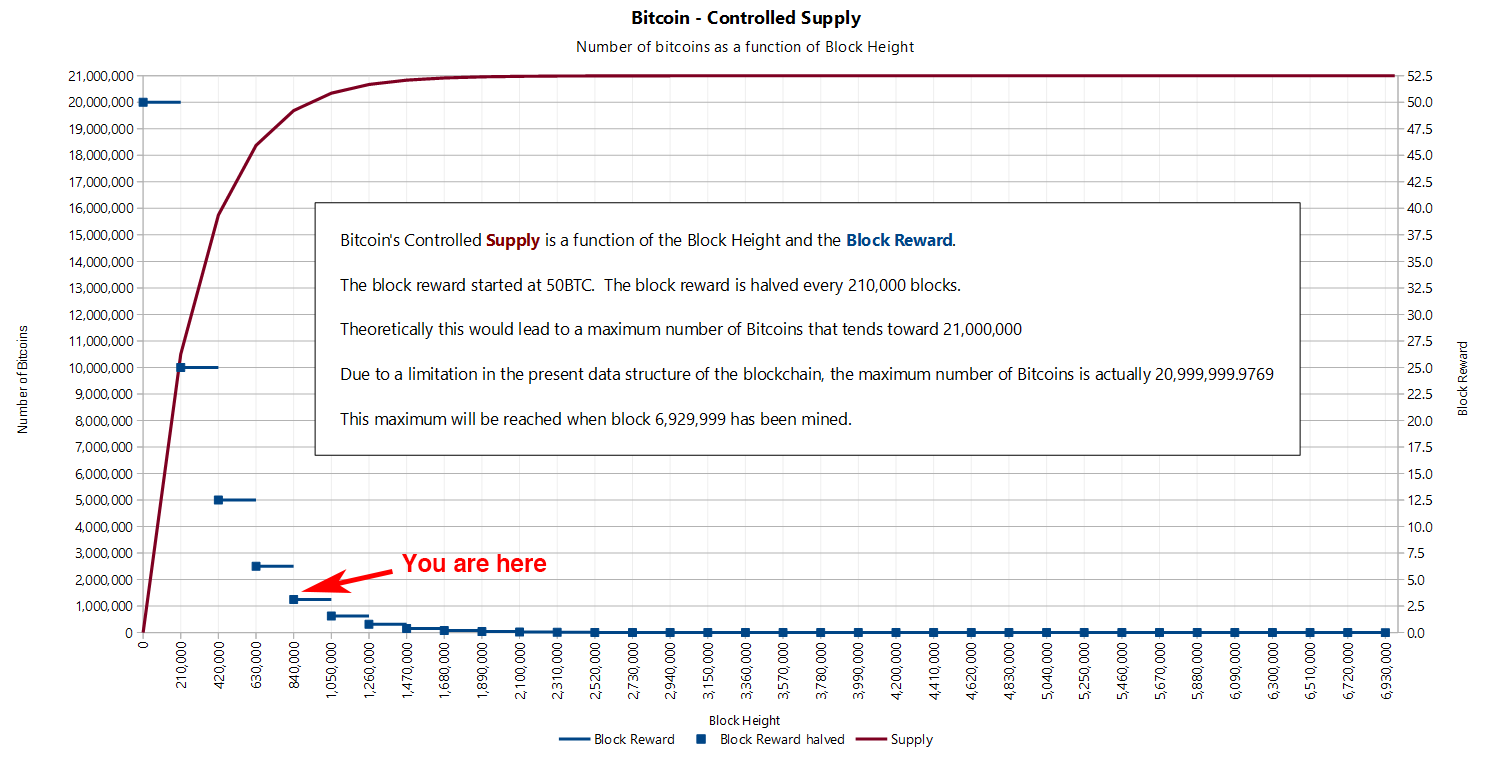
\includegraphics{assets/images/you-are-here.png}
  \caption{Bitcoin's controlled supply}
  \label{fig:you-are-here.png}
\end{figure}

Formulas, logarithmic functions and exponentials are not exactly
intuitive to understand. The concept of \textit{soundness} might be easier to
understand if looked at in another way. Once we know how much there is
of something, and once we know how hard this something is to produce or
get our hands on, we immediately understand its value. What is true for
Picasso's paintings, Elvis Presley's guitars, and Stradivarius violins
is also true for fiat currency, gold, and bitcoins.

The hardness of fiat currency depends on who is in charge of the
respective printing presses. Some governments might be more willing to
print large amounts of currency than others, resulting in a weaker
currency. Other governments might be more restrictive in their money
printing, resulting in harder currency.

\begin{samepage}\begin{quotation}
\enquote{One important aspect of this new reality is that institutions like
the Fed cannot go bankrupt. They can print any amount of money that
they might need for themselves at virtually zero cost.}
\begin{flushright} -- Jörg Guido Hülsmann\footnote{Jörg Guido Hülsmann, \textit{The
Ethics of Money Production}~\cite{hulsmann2008ethics}}
\end{flushright}\end{quotation}\end{samepage}

Before we had fiat currencies, the soundness of money was determined by
the natural properties of the stuff which we used as money. The amount
of gold on earth is limited by the laws of physics. Gold is rare because
supernovae and neutron star collisions are rare. The \enquote{flow} of gold is
limited because extracting it is quite an effort. Being a heavy element
it is mostly buried deep underground.

The abolishment of the gold standard gave way to a new reality: adding new money
requires just a drop of ink. In our modern world adding a couple of zeros to the
balance of a bank account requires even less effort: flipping a few bits in a
bank computer is enough.


The principle outlined above can be expressed more generally as the
ratio of \enquote{stock} to \enquote{flow}. Simply put, the \textit{stock} is how much of
something is currently there. For our purposes, the stock is a measure
of the current money supply. The \textit{flow} is how much there is produced
over a period of time (e.g. per year). The key to understanding sound
money is in understanding this stock-to-flow ratio.

Calculating the stock-to-flow ratio for fiat currency is difficult, because how
much money there is depends on how you look at it.~\cite{wiki:money-supply} You
could count only banknotes and coins (M0), add traveler checks and check
deposits (M1), add saving accounts and mutual funds and some other things (M2),
and even add certificates of deposit to all of that (M3). Further, how all of
this is defined and measured varies from country to country and since the US
Federal Reserve stopped publishing \cite{web:fed-m3} numbers for M3, we will
have to make do with the M2 monetary supply. I would love to verify these
numbers, but I guess we have to trust the fed for now.

Gold, one of the rarest metals on earth, has the highest stock-to-flow
ratio. According to the US Geological Survey, a little more than 190,000
tons have been mined. In the last few years, around 3100 tons of gold
have been mined per year.~\cite{mineral-commodity-summaries}

Using these numbers, we can easily calculate the stock-to-flow ratio for
gold (see Figure~\ref{fig:stock-to-flow-gold}).

\begin{figure}
  \centering
  \begin{equation}
  \frac{190,000 t}{3,100 t} = ~ 61
  \end{equation}
  \caption{Stock-to-flow ratio of gold}
  \label{fig:stock-to-flow-gold}
\end{figure}

Nothing has a higher stock-to-flow ratio than gold. This is why gold, up to now,
was the hardest, soundest money in existence. It is often said that all the gold
mined so far would fit in two olympic-sized swimming pools. According to my
calculations\footnote{\url{https://bit.ly/gold-pools}}, we would need four. So
maybe this needs updating, or Olympic-sized swimming pools got smaller.

Enter Bitcoin. As you probably know, bitcoin mining was all the rage in
the last couple of years. This is because we are still in the early
phases of what is called the \textit{reward era}, where mining nodes are
rewarded with \textit{a lot} of bitcoin for their computational effort. We are
currently in reward era number 3, which began in 2016 and will end in
early 2020, probably in May. While the bitcoin supply is predetermined,
the inner workings of Bitcoin only allow for approximate dates.
Nevertheless, we can predict with certainty how high Bitcoin's
stock-to-flow ratio will be. Spoiler alert: it will be high.

How high? Well, it turns out that Bitcoin will get infinitely hard (see
Figure~\ref{fig:stock-to-flow-white-cropped}).

\begin{figure}
  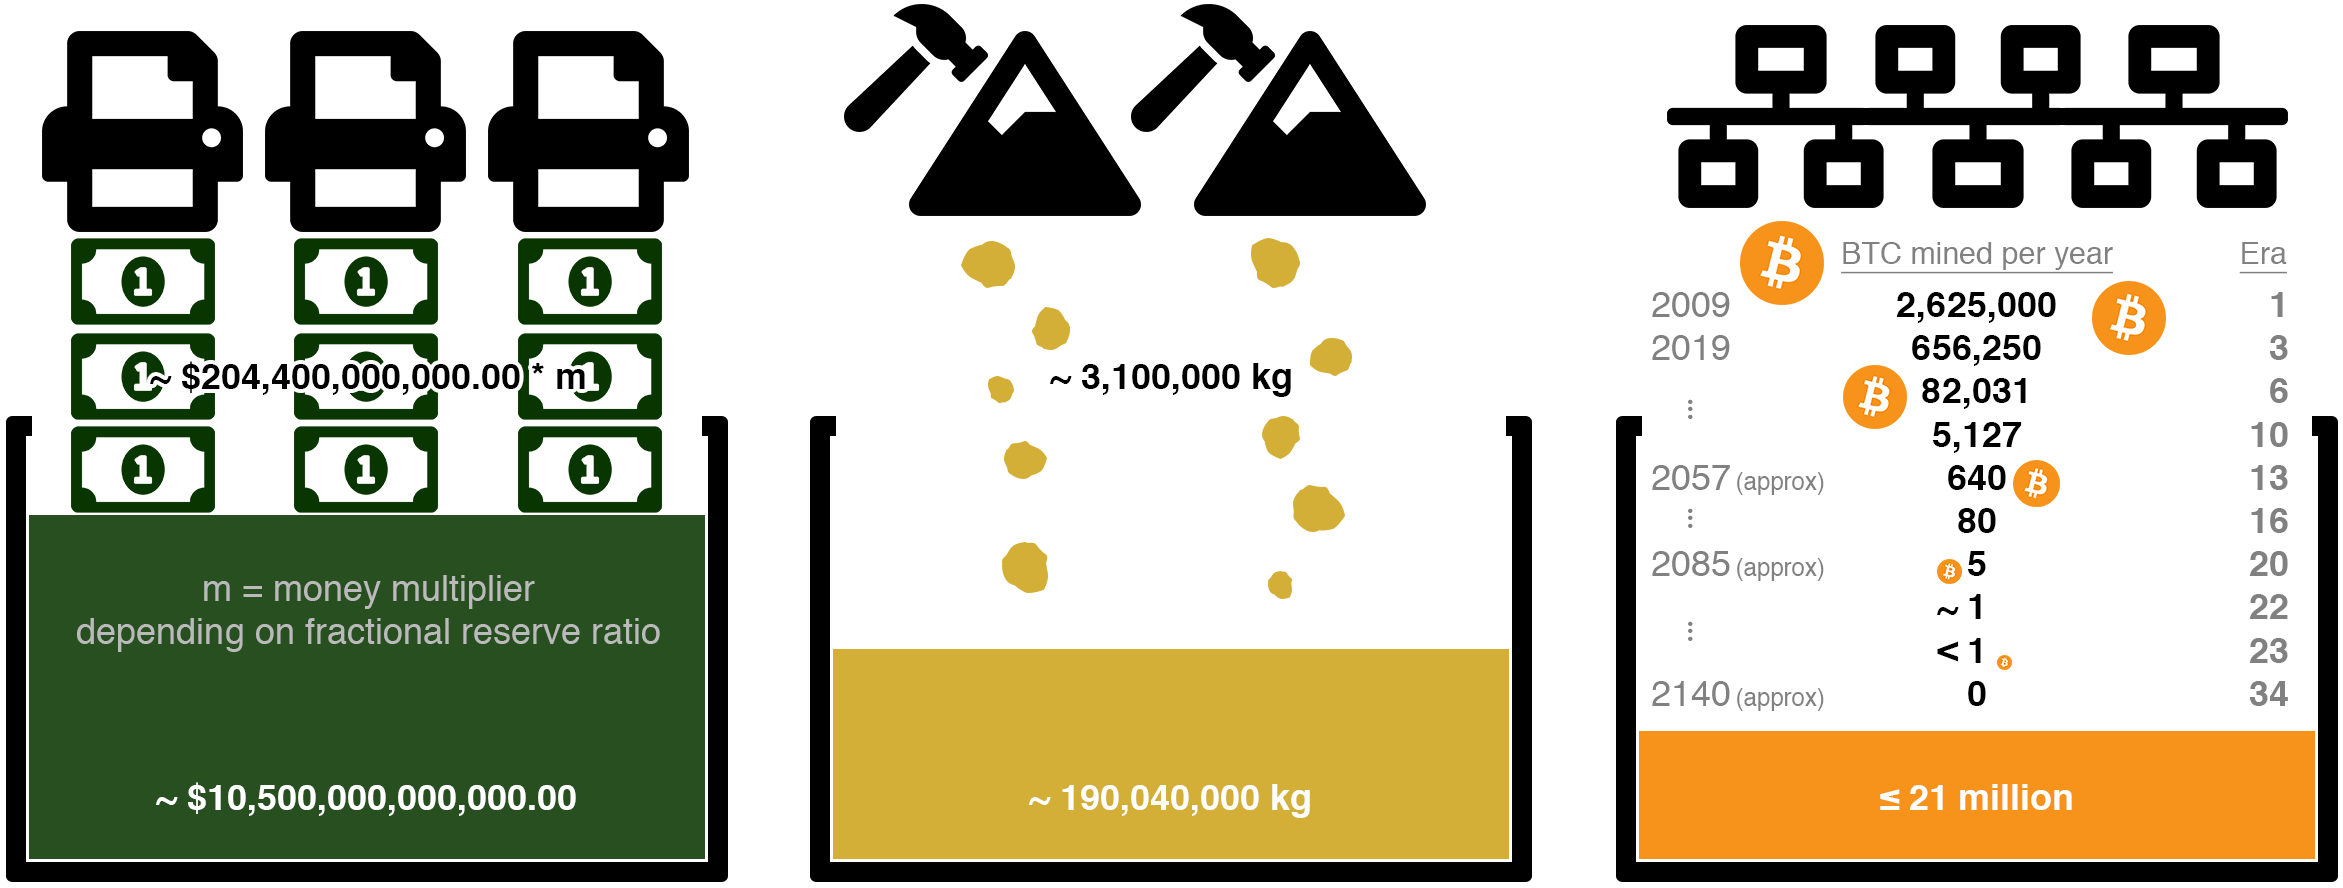
\includegraphics{assets/images/stock-to-flow-white-cropped.png}
  \caption{Visualization of stock and flow for USD, gold, and Bitcoin}
  \label{fig:stock-to-flow-white-cropped}
\end{figure}

\paragraph{}
Due to an exponential decrease of the mining reward, the flow of new
bitcoin will diminish resulting in a sky-rocketing stock-to-flow ratio.
It will catch up to gold in 2020, only to surpass it four years later by
doubling its soundness again. Such a doubling will occur 64 times in
total. Thanks to the power of exponentials, the number of bitcoin mined
per year will drop below 100 bitcoin in 50 years and below 1 bitcoin in
75 years. The global faucet which is the block reward will dry up
somewhere around the year 2140, effectively stopping the production of
bitcoin. This is a long game. If you are reading this, you are still
early.

\begin{figure}
  \includegraphics{assets/images/soundness-over-time.png}
  \caption{Rising stock-to-flow ratio of bitcoin as compared to gold}
  \label{fig:soundness-over-time}
\end{figure}

As bitcoin approaches infinite stock to flow ratio it will be the
soundest money in existence. Infinite soundness is hard to beat.

Viewed through the lens of economics, Bitcoin's \textit{difficulty adjustment}
is probably its most important component. How hard it is to mine bitcoin depends
on how quickly new bitcoins are mined.\footnote{It actually depends on how
quickly valid blocks are found, but for our purposes, this is the same thing as
\enquote{mining bitcoins} and will be so for the next 120 years.} It is the dynamic
adjustment of the network's mining difficulty which enables us to predict its
future supply.

The simplicity of the difficulty adjustment algorithm might distract
from its profundity, but the difficulty adjustment truly is a revolution
of Einsteinian proportions. It ensures that, no matter how much or how
little effort is spent on mining, Bitcoin's controlled supply won't be
disrupted. As opposed to every other resource, no matter how much
energy someone will put into mining bitcoin, the total reward will not
increase.

Just like $E=mc^2$ dictates the universal speed limit in our universe,
Bitcoin's difficulty adjustment dictates the \textbf{universal money limit}
in Bitcoin.

\paragraph{}
If it weren't for this difficulty adjustment, all bitcoins would have been mined
already. If it weren't for this difficulty adjustment, Bitcoin probably wouldn't
have survived in its infancy. It is what secures the network in its reward era.
It is what ensures a steady and fair distribution\footnote{Dan Held,
\textit{Bitcoin's Distribution was Fair}~\cite{distribution-was-fair}} of new
bitcoin. It is the thermostat which regulates Bitcoin's monetary policy.

Einstein showed us something novel: no matter how hard you push an
object, at a certain point you won't be able to get more speed out of
it. Satoshi also showed us something novel: no matter how hard you dig
for this digital gold, at a certain point you won't be able to get more
bitcoin out of it. For the first time in human history, we have a
monetary good which, no matter how hard you try, you won't be able to
produce more of.

\paragraph{Bitcoin taught me that sound money is essential.}

% ---
%
% #### Through the Looking-Glass
%
% - [Bitcoin's Energy Consumption: A Shift in Perspective][much energy]
%
% #### Down the Rabbit Hole
%
% - [The Ethics of Money Production][Jörg Guido Hülsmann] by Jörg Guido Hülsmann
% - [Mineral Commodity Summaries 2019][last few years] by the United States Geological Survey
% - [Bitcoin’s Distribution was Fair][fair distribution] by Dan Held
% - [Bitcoin's Controlled Supply][algorithmically controlled] on the Bitcoin Wiki
% - [Money Supply][how much money there is], [Speed of Light][universal speed limit] on Wikipedia
%
% <!-- Internal -->
% [much energy]: 
%
% [Fr. Bernard W. Dempsey, S.J.]: https://www.jstor.org/stable/29769582
% [Jörg Guido Hülsmann]: https://mises.org/sites/default/files/The%20Ethics%20of%20Money%20Production_2.pdf
% [stopped publishing]: https://www.federalreserve.gov/Releases/h6/discm3.htm
% [last few years]: https://minerals.usgs.gov/minerals/pubs/mcs/2018/mcs2018.pdf
% [my calculations]: https://www.wolframalpha.com/input/?i=volume+of+190000+metric+tons+gold+%2F+olympic+swimming+pool+volume
% [fair distribution]: https://blog.picks.co/bitcoins-distribution-was-fair-e2ef7bbbc892
%
% <!-- Bitcoin Wiki -->
% [algorithmically controlled]: https://en.bitcoin.it/wiki/Controlled_supply
%
% <!-- Wikipedia -->
% [how much money there is]: https://en.wikipedia.org/wiki/Money_supply
% [universal speed limit]: https://en.wikipedia.org/wiki/Speed_of_light#Upper_limit_on_speeds
% [alice]: https://en.wikipedia.org/wiki/Alice%27s_Adventures_in_Wonderland
% [carroll]: https://en.wikipedia.org/wiki/Lewis_Carroll

\part{Tecnologia}
\label{ch:technology}
\chapter*{Tecnologia}

\begin{chapquote}{Lewis Carroll, \textit{Alice no País das Maravilhas}}
\enquote{Desta vez vou me sair melhor}, disse para si mesma, e começou por pegar a chavezinha de ouro e destrancar a porta que dava para o jardim.
\end{chapquote}

Chaves de ouro, relógios que só funcionam por acaso, corridas para resolver enigmas estranhos e construtores que não têm rostos nem nomes. O que parece contos de fadas do País das Maravilhas é um negócio comum no mundo do Bitcoin.

Como exploramos no Capítulo~\ref{ch:economics}, grandes partes do sistema financeiro atual são sistematicamente falhas. Como Alice, só podemos esperar administrar melhor desta vez. Mas, graças a um inventor pseudônimo, temos uma tecnologia incrivelmente sofisticada para nos apoiar desta vez: o Bitcoin.

Resolver problemas em um ambiente radicalmente descentralizado e adversário requer soluções únicas. O que de outra forma seriam problemas triviais para resolver são tudo, menos isso, neste mundo estranho. O Bitcoin depende de uma forte criptografia para a maioria das soluções, pelo menos quando analisado através das lentes da tecnologia. Iremos explorar o quão forte essa criptografia é, em uma das lições a seguir.

A criptografia é o que o Bitcoin usa para remover a confiança nas autoridades. Ao invés de depender de instituições centralizadas, o sistema depende da autoridade final do nosso universo: a física. Alguns pequenos grãos de confiança ainda são necessários, no entanto. Examinaremos esses grãos na segunda lição deste capítulo.

~

\begin{samepage}
Parte~\ref{ch:technology} -- Tecnologia:

\begin{enumerate}
  \setcounter{enumi}{14}
  \item Força nos números
  \item Reflexos no \enquote{Não Confie, Verifique}
  \item Dizer o tempo demanda trabalho
  \item Mova-se lentamente e não quebre as coisas
  \item Privacidade não está morta
  \item Cypherpunks escrevem códigos
  \item Metáforas para um futuro do Bitcoin
\end{enumerate}
\end{samepage}

As últimas duas lições exploram o \textit{ethos} do desenvolvimento tecnológico no Bitcoin, que é indiscutivelmente tão importante quanto a própria tecnologia. O Bitcoin não é o próximo aplicativo revolucionário no seu celular. É a base de uma nova realidade econômica, razão pela qual o Bitcoin deve ser tratado como um software financeiro de nível nuclear.

Onde estamos nesta revolução financeira, social e tecnológica? Redes e tecnologias do passado podem servir como metáforas para o futuro dos Bitcoins, que são exploradas na última lição deste capítulo.

Mais uma vez, aperte o cinto e aproveite o passeio. Como todas as tecnologias exponenciais, estamos prestes a nos tornar parabólicos.
\chapter{Strength in Numbers}
\label{les:15}

\begin{chapquote}{Lewis Carroll, \textit{Alice in Wonderland}}
\enquote{Let me see: four times five is twelve, and four times six is thirteen, and
four times seven is fourteen—oh dear! I shall never get to twenty at this
rate!}
\end{chapquote}

Numbers are an essential part of our everyday life. Large numbers,
however, aren't something most of us are too familiar with. The largest
numbers we might encounter in everyday life are in the range of
millions, billions, or trillions. We might read about millions of people
in poverty, billions of dollars spent on bank bailouts, and trillions of
national debt. Even though it's hard to make sense of these headlines,
we are somewhat comfortable with the size of those numbers.

Although we might seem comfortable with billions and trillions, our
intuition already starts to fail with numbers of this magnitude. Do you
have an intuition how long you would have to wait for a
million/billion/trillion seconds to pass? If you are anything like me,
you are lost without actually crunching the numbers.

Let's take a closer look at this example: the difference between each is an
increase by three orders of magnitude: $10^6$, $10^9$, $10^{12}$. Thinking about
seconds is not very useful, so let's translate this into something we can wrap
our head around:

\begin{itemize}
  \item $10^6$: One million seconds was $1 1/2$ weeks ago.
  \item $10^9$: One billion seconds was almost 32 years ago.
  \item $10^{12}$: One trillion seconds ago Manhattan was covered under a thick
  layer of ice.\footnote{One trillion seconds ($10^{12}$) was $31710$ years ago. The Last Glacial
  Maximum was $33,000$ years ago.~\cite{wiki:LGM}}
\end{itemize}

\begin{figure}
  \includegraphics[width=\textwidth]{assets/images/xkcd-1225.png}
  \caption{About 1 trillion seconds ago. Source: xkcd 1225}
  \label{fig:xkcd-1225}
\end{figure}

As soon as we enter the beyond-astronomical realm of modern
cryptography, our intuition fails catastrophically. Bitcoin is built
around large numbers and the virtual impossibility of guessing them.
These numbers are way, way larger than anything we might encounter in
day-to-day life. Many orders of magnitude larger. Understanding how
large these numbers truly are is essential to understanding Bitcoin as a
whole.

Let's take SHA-256\footnote{SHA-256 is part of the SHA-2 family of cryptographic
hash functions developed by the NSA.~\cite{wiki:sha2}}, one of the hash
functions\footnote{Bitcoin uses SHA-256 in its block hashing
algorithm.~\cite{btcwiki:block-hashing}} used in Bitcoin, as a concrete example.
It is only natural to think about 256 bits as \enquote{two hundred fifty-six,} which
isn't a large number at all. However, the number in SHA-256 is talking about
orders of magnitude --- something our brains are not well-equipped to deal with.

While bit length is a convenient metric, the true meaning of 256-bit
security is lost in translation. Similar to the millions ($10^6$) and
billions ($10^9$) above, the number in SHA-256 is about orders of magnitude
($2^{256}$).

So, how strong is SHA-256, exactly?

\begin{quotation}\begin{samepage}
\enquote{SHA-256 is very strong. It's not like the incremental step from MD5
to SHA1. It can last several decades unless there's some massive
breakthrough attack.}
\begin{flushright} -- Satoshi Nakamoto\footnote{Satoshi Nakamoto, in a reply to questions about SHA-256 collisions. \cite{satoshi-sha256}}
\end{flushright}\end{samepage}\end{quotation}

Let's spell things out. $2^{256}$ equals the following number:

\begin{quotation}\begin{samepage}
    115 quattuorvigintillion 792 trevigintillion 89 duovigintillion 237
    unvigintillion 316 vigintillion 195 novemdecillion 423 octodecillion 570
    septendecillion 985 sexdecillion 8 quindecillion 687 quattuordecillion 907
    tredecillion 853 duodecillion 269 undecillion 984 decillion 665 nonillion
    640 octillion 564 septillion 39 sextillion 457 quintillion 584 quadrillion 7
    trillion 913 billion 129 million 639 thousand 936.
\end{samepage}\end{quotation}

That's a lot of nonillions! Wrapping your head around this number is
pretty much impossible. There is nothing in the physical universe to
compare it to. It is far larger than the number of atoms in the
observable universe. The human brain simply isn't made to make sense of
it.

\newpage

One of the best visualizations of the true strength of SHA-256 is a video by
Grant Sanderson. Aptly named \textit{\enquote{How secure is 256 bit
security?}}\footnote{Watch the video at \url{https://youtu.be/S9JGmA5_unY}} it
beautifully shows how large a 256-bit space is. Do yourself a favor and take the
five minutes to watch it. As all other \textit{3Blue1Brown} videos it is not
only fascinating but also exceptionally well made. Warning: You might fall down
a math rabbit hole.

\begin{figure}
  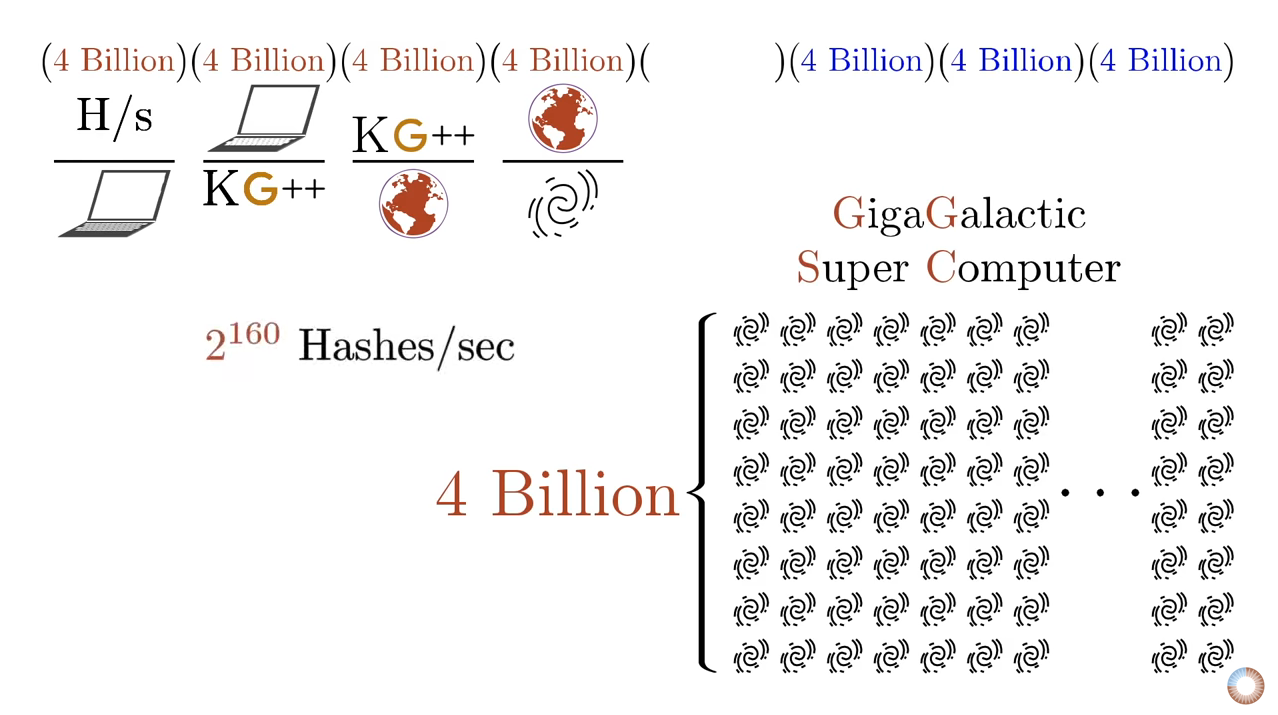
\includegraphics[width=\textwidth]{assets/images/youtube-vid-inverted.png}
  \caption{Illustration of SHA-256 security. Original graphic by Grant Sanderson aka 3Blue1Brown.}
  \label{fig:youtube-vid-inverted}
\end{figure}

Bruce Schneier~\cite{web:schneier} used the physical limits of computation to put this
number into perspective: even if we could build an optimal computer,
which would use any provided energy to flip bits perfectly~\cite{wiki:landauer}, build a
Dyson sphere\footnote{A Dyson sphere is a hypothetical megastructure that completely encompasses a star and captures a large percentage of its power output.~\cite{wiki:dyson}} around our sun, and let it run for 100 billion billion
years, we would still only have a $25\%$ chance to find a needle in a
256-bit haystack.

\begin{quotation}\begin{samepage}
\enquote{These numbers have nothing to do with the technology of the devices;
they are the maximums that thermodynamics will allow. And they
strongly imply that brute-force attacks against 256-bit keys will be
infeasible until computers are built from something other than matter
and occupy something other than space.}
\begin{flushright} -- Bruce Schneier\footnote{Bruce Schneier, \textit{Applied Cryptography} \cite{bruce-schneier}}
\end{flushright}\end{samepage}\end{quotation}


It is hard to overstate the profoundness of this. Strong cryptography
inverts the power-balance of the physical world we are so used to.
Unbreakable things do not exist in the real world. Apply enough force,
and you will be able to open any door, box, or treasure chest.

Bitcoin's treasure chest is very different. It is secured by strong
cryptography, which does not give way to brute force. And as long as the
underlying mathematical assumptions hold, brute force is all we have.
Granted, there is also the option of a global \$5 wrench attack (Figure~\ref{fig:xkcd-538})
But torture won't work for all bitcoin addresses, and the cryptographic
walls of bitcoin will defeat brute force attacks. Even if you come at it
with the force of a thousand suns. Literally.

\begin{figure}
  \centering
  \includegraphics[width=8cm]{assets/images/xkcd-538.png}
  \caption{\$5 wrench attack. Source: xkcd 538}
  \label{fig:xkcd-538}
\end{figure}

This fact and its implications were poignantly summarized in the call
to cryptographic arms: \textit{\enquote{No amount of coercive force will ever solve
a math problem.}}

\begin{quotation}\begin{samepage}
\enquote{It isn't obvious that the world had to work this way. But somehow the
universe smiles on encryption.}
\begin{flushright} -- Julian Assange\footnote{Julian Assange, \textit{A Call to Cryptographic Arms} \cite{call-to-cryptographic-arms}}
\end{flushright}\end{samepage}\end{quotation}

Nobody yet knows for sure if the universe's smile is genuine or not. It
is possible that our assumption of mathematical asymmetries is wrong and
we find that P actually equals NP \cite{wiki:pnp}, or we find surprisingly quick
solutions to specific problems \cite{wiki:discrete-log} which we currently assume to be hard.
If that should be the case, cryptography as we know it will cease to
exist, and the implications would most likely change the world beyond
recognition.

\begin{quotation}\begin{samepage}
\enquote{Vires in Numeris} = \enquote{Strength in Numbers}\footnote{\textit{Vires in Numeris} was first proposed as a Bitcoin motto by the bitcointalk user \textit{epii}~\cite{epii}}
\end{samepage}\end{quotation}

\textit{Vires in numeris} is not only a catchy motto used by bitcoiners. The
realization that there is an unfathomable strength to be found in
numbers is a profound one. Understanding this, and the inversion of
existing power balances which it enables changed my view of the world
and the future which lies ahead of us.

One direct result of this is the fact that you don't have to ask anyone
for permission to participate in Bitcoin. There is no page to sign up,
no company in charge, no government agency to send application forms to.
Simply generate a large number and you are pretty much good to go. The
central authority of account creation is mathematics. And God only knows
who is in charge of that.

\begin{figure}
  \includegraphics[width=\textwidth]{assets/images/elliptic-curve-examples.png}
  \caption{Elliptic curve examples. Graphic cc-by-sa Emmanuel Boutet.}
  \label{fig:elliptic-curve-examples}
\end{figure}

Bitcoin is built upon our best understanding of reality. While there are
still many open problems in physics, computer science, and mathematics,
we are pretty sure about some things. That there is an asymmetry between
finding solutions and validating the correctness of these solutions is
one such thing. That computation needs energy is another one. In other
words: finding a needle in a haystack is harder than checking if the
pointy thing in your hand is indeed a needle or not. And finding the
needle takes work.

The vastness of Bitcoin's address space is truly mind-boggling. The
number of private keys even more so. It is fascinating how much of our
modern world boils down to the improbability of finding a needle in an
unfathomably large haystack. I am now more aware of this fact than ever.

\paragraph{Bitcoin taught me that there is strength in numbers.}

% ---
%
% #### Down the Rabbit Hole
%
% - [How secure is 256 bit security?]["How secure is 256 bit security?"] by 3Blue1Brown
% - [Block Hashing Algorithm][hash functions] on the Bitcoin Wiki
% - [Last Glacial Maximum][thick layer of ice], [SHA-2][SHA-256], [Dyson Sphere][Dyson sphere], [Landauer's Principle][flip bits perfectly] [P versus NP][P actually equals NP], [Discrete Logarithm][specific problems] on Wikipedia
%
% [thick layer of ice]: https://en.wikipedia.org/wiki/Last_Glacial_Maximum
% [xkcd \#1125]: https://xkcd.com/1225/
% [SHA-256]: https://en.wikipedia.org/wiki/SHA-2
% [hash functions]: https://en.bitcoin.it/wiki/Block_hashing_algorithm
% ["How secure is 256 bit security?"]: https://www.youtube.com/watch?v=S9JGmA5_unY
% [Bruce Schneier]: https://www.schneier.com/
% [flip bits perfectly]: https://en.wikipedia.org/wiki/Landauer%27s_principle#Equation
% [Dyson sphere]: https://en.wikipedia.org/wiki/Dyson_sphere
% [2]: https://books.google.com/books?id=Ok0nDwAAQBAJ&pg=PT316&dq=%22These+numbers+have+nothing+to+do+with+the+technology+of+the+devices;%22&hl=en&sa=X&ved=0ahUKEwjXttWl8YLhAhUphOAKHZZOCcsQ6AEIKjAA#v=onepage&q&f=false
% [wrench attack]: https://xkcd.com/538/
% [call to cryptographic arms]: https://cryptome.org/2012/12/assange-crypto-arms.htm
% [P actually equals NP]: https://en.wikipedia.org/wiki/P_versus_NP_problem#P_=_NP
% [specific problems]: https://en.wikipedia.org/wiki/Discrete_logarithm#Cryptography
% [3Blue1Brown]: https://twitter.com/3blue1brown
%
% <!-- Wikipedia -->
% [alice]: https://en.wikipedia.org/wiki/Alice%27s_Adventures_in_Wonderland
% [carroll]: https://en.wikipedia.org/wiki/Lewis_Carroll

\chapter{Reflections on \enquote{Don't Trust, Verify}}
\label{les:16}

\begin{chapquote}{Lewis Carroll, \textit{Alice in Wonderland}}
\enquote{Now for the evidence,} said the King, \enquote{and then the sentence.}
\end{chapquote}

Bitcoin aims to replace, or at least provide an alternative to,
conventional currency. Conventional currency is bound to a centralized
authority, no matter if we are talking about legal tender like the US
dollar or modern monopoly money like Fortnite's V-Bucks. In both
examples, you are bound to trust the central authority to issue, manage
and circulate your money. Bitcoin unties this bound, and the main issue
Bitcoin solves is the issue of \textit{trust}.

\begin{quotation}\begin{samepage}
\enquote{The root problem with conventional currency is all the trust that's
required to make it work. [...] What is needed is an electronic
payment system based on cryptographic proof instead of trust}
\begin{flushright} -- Satoshi Nakamoto\footnote{Satoshi Nakamoto, official Bitcoin announcement~\cite{bitcoin-announcement} and whitepaper~\cite{whitepaper}}
\end{flushright}\end{samepage}\end{quotation}

Bitcoin solves the problem of trust by being completely decentralized,
with no central server or trusted parties. Not even trusted \textit{third}
parties, but trusted parties, period. When there is no central
authority, there simply \textit{is} no-one to trust. Complete decentralization
is the innovation. It is the root of Bitcoin's resilience, the reason
why it is still alive. Decentralization is also why we have mining,
nodes, hardware wallets, and yes, the blockchain. The only thing you
have to \enquote{trust} is that our understanding of mathematics and physics
isn't totally off and that the majority of miners act honestly (which
they are incentivized to do).

While the regular world operates under the assumption of \textit{\enquote{trust,
but verify,}} Bitcoin operates under the assumption of \textit{\enquote{don't
trust, verify.}} Satoshi made the importance of removing trust very clear in
both the introduction as well as the conclusion of the Bitcoin whitepaper.

\begin{quotation}\begin{samepage}
\enquote{Conclusion: We have proposed a system for electronic transactions
without relying on trust.}
\begin{flushright} -- Satoshi Nakamoto\footnote{Satoshi Nakamoto, the Bitcoin whitepaper~\cite{whitepaper}}
\end{flushright}\end{samepage}\end{quotation}

Note that \textit{without relying on trust} is used in a very specific context
here. We are talking about trusted third parties, i.e. other entities
which you trust to produce, hold, and process your money. It is assumed,
for example, that you can trust your computer.

As Ken Thompson showed in his Turing Award lecture, trust is an
extremely tricky thing in the computational world. When running a
program, you have to trust all kinds of software (and hardware) which,
in theory, could alter the program you are trying to run in a malicious
way. As Thompson summarized in his \textit{Reflections on Trusting Trust}:
\enquote{The moral is obvious. You can't trust code that you did not totally
create yourself.}~\cite{trusting-trust}

\begin{figure}
  \includegraphics[width=\textwidth]{assets/images/ken-thompson-hack.png}
  \caption{Excerpts from Ken Thompson's paper `Reflections on Trusting Trust'}
  \label{fig:ken-thompson-hack}
\end{figure}

Thompson demonstrated that even if you have access to the source code,
your compiler --- or any other program-handling program or
hardware --- could be compromised and detecting this backdoor would be
very difficult. Thus, in practice, a truly \textit{trustless} system does not
exist. You would have to create all your software \textit{and} all your
hardware (assemblers, compilers, linkers, etc.) from scratch, without
the aid of any external software or software-aided machinery.

\begin{quotation}\begin{samepage}
\enquote{If you wish to make an apple pie from scratch, you must first invent
the universe.}
\begin{flushright} -- Carl Sagan\footnote{Carl Sagan, \textit{Cosmos} \cite{cosmos}}
\end{flushright}\end{samepage}\end{quotation}

The Ken Thompson Hack is a particularly ingenious and hard-to-detect backdoor,
so let's take a quick look at a hard-to-detect backdoor which works without
modifying any software. Researchers found a way to compromise security-critical
hardware by altering the polarity of silicon
impurities.~\cite{becker2013stealthy} Just by changing the physical properties
of the stuff that computer chips are made of they were able to compromise a
cryptographically secure random number generator. Since this change can't be
seen, the backdoor can't be detected by optical inspection, which is one of the
most important tamper-detection mechanism for chips like these.

\begin{figure}
  \includegraphics[width=\textwidth]{assets/images/stealthy-hardware-trojan.png}
  \caption{Stealthy Dopant-Level Hardware Trojans by Becker, Regazzoni, Paar, Burleson}
  \label{fig:stealthy-hardware-trojan}
\end{figure}

Sounds scary? Well, even if you would be able to build everything from
scratch, you would still have to trust the underlying mathematics. You
would have to trust that \textit{secp256k1} is an elliptic curve without
backdoors. Yes, malicious backdoors can be inserted in the mathematical
foundations of cryptographic functions and arguably this has already
happened at least once.~\cite{wiki:Dual_EC_DRBG} There are good reasons to be paranoid, and the
fact that everything from your hardware, to your software, to the
elliptic curves used can have backdoors~\cite{wiki:backdoors} are some of them.

\begin{quotation}\begin{samepage}
\enquote{Don't trust. Verify.}
\begin{flushright} -- Bitcoiners everywhere
\end{flushright}\end{samepage}\end{quotation}

The above examples should illustrate that \textit{trustless} computing is
utopic. Bitcoin is probably the one system which comes closest to this
utopia, but still, it is \textit{trust-minimized} --- aiming to remove trust
wherever possible. Arguably, the chain-of-trust is neverending, since
you will also have to trust that computation requires energy, that P
does not equal NP, and that you are actually in base reality and not
imprisoned in a simulation by malicious actors.

Developers are working on tools and procedures to minimize any remaining trust
even further. For example, Bitcoin developers created
Gitian\footnote{\url{https://gitian.org/}}, which is a software distribution
method to create deterministic builds. The idea is that if multiple developers
are able to reproduce identical binaries, the chance of malicious tampering is
reduced. Fancy backdoors aren't the only attack vector. Simple blackmail or
extortion are real threats as well. As in the main protocol, decentralization is
used to minimize trust.

Various efforts are being made to improve upon the chicken-and-egg problem of
bootstrapping which Ken Thompson's hack so brilliantly pointed
out~\cite{web:bootstrapping}. One such effort is
Guix\footnote{\url{https://guix.gnu.org}} (pronounced \textit{geeks}), which
uses functionally declared package management leading to bit-for-bit
reproducible builds by design. The result is that you don't have to trust any
software-providing servers anymore since you can verify that the served binary
was not tampered with by rebuilding it from scratch. Recently, a
pull-request was merged to integrate Guix into the Bitcoin build process.\footnote{See PR 15277 of \texttt{bitcoin-core}: \\ \url{https://github.com/bitcoin/bitcoin/pull/15277}}

\begin{figure}
  \includegraphics[width=\textwidth]{assets/images/guix-bootstrap-dependencies.png}
  \caption{Which came first, the chicken or the egg?}
  \label{fig:guix-bootstrap-dependencies}
\end{figure}

Luckily, Bitcoin doesn't rely on a single algorithm or piece of
hardware. One effect of Bitcoin's radical decentralization is a
distributed security model. Although the backdoors described above are
not to be taken lightly, it is unlikely that every software wallet,
every hardware wallet, every cryptographic library, every node
implementation, and every compiler of every language is compromised.
Possible, but highly unlikely.

Note that you can generate a private key without relying on any computational
hardware or software. You can flip a coin~\cite{antonopoulos2014mastering} a
couple of times, although depending on your coin and tossing style this source
of randomness might not be sufficiently random. There is a reason why storage
protocols like Glacier\footnote{\url{https://glacierprotocol.org/}} advise to
use casino-grade dice as one of two sources of entropy.

Bitcoin forced me to reflect on what trusting nobody actually entails.
It raised my awareness of the bootstrapping problem, and the implicit
chain-of-trust in developing and running software. It also raised my
awareness of the many ways in which software and hardware can be
compromised.

\paragraph{Bitcoin taught me not to trust, but to verify.}

% ---
%
% #### Down the Rabbit Hole
%
% - [The Bitcoin whitepaper][Nakamoto] by Satoshi Nakamoto
% - [Reflections on Trusting Trust][\textit{Reflections on Trusting Trust}] by Ken Thompson
% - [51% Attack][majority] on the Bitcoin Developer Guide
% - [Bootstrapping][bootstrapping], Guix Manual
% - [Secp256k1][secp256k1] on the Bitcoin Wiki
% - [ECC Backdoors][backdoors], [Dual EC DRBG][has already happened] on Wikipedia
%
% [Emmanuel Boutet]: https://commons.wikimedia.org/wiki/User:Emmanuel.boutet
% [\textit{Reflections on Trusting Trust}]: https://www.archive.ece.cmu.edu/~ganger/712.fall02/papers/p761-thompson.pdf
% [found a way]: https://scholar.google.com/scholar?hl=en&as_sdt=0%2C5&q=Stealthy+Dopant-Level+Hardware+Trojans&btnG=
% [Gitian]: https://gitian.org/
% [bootstrapping]: https://www.gnu.org/software/guix/manual/en/html_node/Bootstrapping.html
% [Guix]: https://www.gnu.org/software/guix/
% [pull-request]: https://github.com/bitcoin/bitcoin/pull/15277
% [flip a coin]: https://github.com/bitcoinbook/bitcoinbook/blob/develop/ch04.asciidoc#private-keys
% [Glacier]: https://glacierprotocol.org/
% [secp256k1]: https://en.bitcoin.it/wiki/Secp256k1
% [majority]: https://bitcoin.org/en/developer-guide#term-51-attack
%
% <!-- Wikipedia -->
% [backdoors]: https://en.wikipedia.org/wiki/Elliptic-curve_cryptography#Backdoors
% [has already happened]: https://en.wikipedia.org/wiki/Dual_EC_DRBG
% [Carl Sagan]: https://en.wikipedia.org/wiki/Cosmos_%28Carl_Sagan_book%29
% [alice]: https://en.wikipedia.org/wiki/Alice%27s_Adventures_in_Wonderland
% [carroll]: https://en.wikipedia.org/wiki/Lewis_Carroll

\chapter{Telling Time Takes Work}
\label{les:17}

\begin{chapquote}{Lewis Carroll, \textit{Alice in Wonderland}}
\enquote{Dear, dear! I shall be too late!}
\end{chapquote}

It is often said that bitcoins are mined because thousands of computers
work on solving \textit{very complex} mathematical problems. Certain problems
are to be solved, and if you compute the right answer, you \enquote{produce} a
bitcoin. While this simplified view of bitcoin mining might be easier to
convey, it does miss the point somewhat. Bitcoins aren't produced or
created, and the whole ordeal is not really about solving particular
math problems. Also, the math isn't particularly complex. What is
complex is \textit{telling the time} in a decentralized system.

As outlined in the whitepaper, the proof-of-work system (aka mining) is
a way to implement a distributed timestamp server.

\begin{center}
  \includegraphics[width=\textwidth]{assets/images/bitcoin-whitepaper-timestamp-wide.png}
  \captionof{figure}{Excerpts from the whitepaper. Did someone say timechain?}
  \label{fig:bitcoin-whitepaper-timestamp-wide}
\end{center}

When I first learned how Bitcoin works I also thought that proof-of-work
is inefficient and wasteful. After a while, I started to shift my
perspective on Bitcoin's energy consumption~\cite{gigi:energy}. It seems that
proof-of-work is still widely misunderstood today, in the year 10 AB
(after Bitcoin).

Since the problems to be solved in proof-of-work are made up, many
people seem to believe that it is \textit{useless} work. If the focus is purely
on the computation, this is an understandable conclusion. But Bitcoin
isn't about computation. It is about \textit{independently agreeing on the
order of things.}

Proof-of-work is a system in which everyone can validate what happened
and in what order it happened. This independent validation is what leads
to consensus, an individual agreement by multiple parties about who owns
what.

In a radically decentralized environment, we don't have the luxury of absolute
time. Any clock would introduce a trusted third party, a central point in the
system which had to be relied upon and could be attacked. \enquote{Timing is the root
problem,} as Grisha Trubetskoy points out~\cite{pow-clock}. And Satoshi
brilliantly solved this problem by implementing a decentralized clock via a
proof-of-work blockchain. Everyone agrees beforehand that the chain with the
most cumulative work is the source of truth. It is per definition what actually
happened. This agreement is what is now known as Nakamoto consensus.

\begin{quotation}\begin{samepage}
\enquote{The network timestamps transactions by hashing them into an ongoing
chain which serves as proof of the sequence of events witnessed}
\begin{flushright} -- Satoshi Nakamoto\footnote{Satoshi Nakamoto, the Bitcoin whitepaper~\cite{whitepaper}}
\end{flushright}\end{samepage}\end{quotation}

Without a consistent way to tell the time, there is no consistent way to
tell before from after. Reliable ordering is impossible. As mentioned
above, Nakamoto consensus is Bitcoin's way to consistently tell the
time. The system's incentive structure produces a probabilistic,
decentralized clock, by utilizing both greed and self-interest of
competing participants. The fact that this clock is imprecise is
irrelevant because the order of events is eventually unambiguous and can
be verified by anyone.

Thanks to proof-of-work, both the work \textit{and} the validation of the work
are radically decentralized. Everyone can join and leave at will, and
everyone can validate everything at all times. Not only that, but
everyone can validate the state of the system \textit{individually}, without
having to rely on anyone else for validation.

Understanding proof-of-work takes time. It is often counter-intuitive,
and while the rules are simple, they lead to quite complex phenomena.
For me, shifting my perspective on mining helped. Useful, not useless.
Validation, not computation. Time, not blocks.

\paragraph{Bitcoin taught me that telling the time is tricky, especially if you are
decentralized.}

% ---
%
% #### Through the Looking-Glass
%
% - [Bitcoin's Energy Consumption: A shift in perspective][energy]
%
% #### Down the Rabbit Hole
%
% - [Blockchain Proof-of-Work Is a Decentralized Clock][points out] by Gregory Trubetskoy
% - [The Anatomy of Proof-of-Work][pow-anatomy] by Hugo Nguyen
% - [PoW is efficient][pow-efficient] by Dan Held
% - [Mining][bw-mining], [Controlled supply][bw-supply] on the Bitcoin Wiki
%
% [points out]: https://grisha.org/blog/2018/01/23/explaining-proof-of-work/
% [energy]: 
% [whitepaper]: https://bitcoin.org/bitcoin.pdf
%
% [pow-efficient]: https://blog.picks.co/pow-is-efficient-aa3d442754d3
% [pow-anatomy]: https://bitcointechtalk.com/the-anatomy-of-proof-of-work-98c85b6f6667
% [bw-mining]: https://en.bitcoin.it/wiki/Mining
% [bw-supply]: https://en.bitcoin.it/wiki/Controlled_supply
%
% <!-- Wikipedia -->
% [alice]: https://en.wikipedia.org/wiki/Alice%27s_Adventures_in_Wonderland
% [carroll]: https://en.wikipedia.org/wiki/Lewis_Carroll

\chapter{Mova-se lentamente e não quebre as coisas}
\label{les:18}

\begin{chapquote}{Lewis Carroll, \textit{Alice no País das Maravilhas}}
Assim, o barco navegou lentamente, sob o brilhante dia de verão, com sua tripulação alegre e sua música de vozes e risos\footnote{Nota do tradutor: Esse trecho da Alice no País das Maravilhas não foi encontrada em nenhuma das edições utilizadas na tradução, por isso foi feita a tradução do texto incluído pelo autor.}\ldots
\end{chapquote}

Pode ser um mantra esquecido, mas \enquote{move-se rápido e quebrar as coisas} ainda é o \textit{modus operandi} da tecnologia contemporânea. A ideia de que, não importa se você acertar tudo na primeira vez, é um pilar básico da mentalidade \textit{falhe cedo, falhe frequentemente}. O sucesso é medido pelo crescimento, então, enquanto você está crescendo, tudo bem. Se algo não funcionar no início, você simplesmente faz o pivoteamento e itera. Em outras palavras: jogue merda no ventilador e veja qual que gruda.

O Bitcoin é muito diferente. É diferente por design. É diferente por necessidade. Como Satoshi apontou, a moeda eletrônica já foi tentada muitas vezes anteriormente, e todas as tentativas falharam porque os desenvolvedores criavam uma fera que tinha uma cabeça para ser cortada. A novidade do Bitcoin, é que ele é uma besta sem cabeça.

\begin{quotation}\begin{samepage}
\enquote{Muitas pessoas descartam automaticamente a moeda eletrônica como uma causa perdida
por conta de todas as empresas que faliram desde a década de 1990. Espero que seja
óbvio que foi apenas a natureza centralizada dos sistemas que fizeram com que elas estivessem condenadas.}
\begin{flushright} -- Satoshi Nakamoto\footnote{Satoshi Nakamoto, em resposta ao usuário Sepp Hasslberger. \cite{satoshi-centralized-nature}}
\end{flushright}\end{samepage}\end{quotation}

Uma consequência dessa descentralização radical é uma resistência inerente à mudança. \enquote{Mova-se rápido e quebre as coisas} não funciona e nunca funcionará na camada base do Bitcoin. Mesmo que fosse desejável, não seria possível convencer \textit{todos} os usuários a mudarem seus hábitos. Isso é consenso distribuído. Essa é a natureza do Bitcoin.

\begin{quotation}\begin{samepage}
\enquote{A natureza do Bitcoin é tal que, uma vez que a versão 0.1 foi lançada, o projeto principal foi gravado em pedra para o resto de sua vida.}
\begin{flushright} -- Satoshi Nakamoto\footnote{Satoshi Nakamoto, em resposta ao usuário Gavin Andresen \cite{satoshi-centralized-nature}}
\end{flushright}\end{samepage}\end{quotation}

Esta é uma das muitas propriedades paradoxais do Bitcoin. Todos nós acreditamos que qualquer coisa que seja software pode ser alterada facilmente. Mas a natureza da besta torna muito difícil mudá-la.

Como Hasu mostra lindamente em Abrindo o Contrato Social do Bitcoin~\cite{contrato-social}, mudar as regras do Bitcoin só é possível \textit{propondo} uma mudança e, consequentemente, \textit{convencendo} todos os usuários do Bitcoin a adotarem essa mudança. Isso torna o Bitcoin muito resistente a alterações, mesmo sendo um software.

Essa resiliência é uma das propriedades mais importantes do Bitcoin. Os sistemas de software críticos têm que ser antifrágeis. É isso que a interação da camada social do Bitcoin e sua camada técnica garantem. Os sistemas monetários são adversários por natureza e, como sabemos há milhares de anos, bases sólidas são essenciais em um ambiente hostil.

\begin{quotation}\begin{samepage}
\enquote{E desceu a chuva, e correram rios, e assopraram ventos, e combateram aquela casa, e não caiu, porque estava edificada sobre a rocha.}
\begin{flushright} -- Matheus 7:24--27
\end{flushright}\end{samepage}\end{quotation}

Indiscutivelmente, nesta parábola dos construtores sábios e tolos, o Bitcoin não é a casa. É a rocha. Imutável, imóvel, fornecendo a base para um novo sistema financeiro.

Assim como os geólogos, que sabem que as formações rochosas estão sempre se movendo e evoluindo, pode-se ver que o Bitcoin está sempre se movendo e evoluindo também. Você só precisa saber para onde olhar e como olhar para ele.

A introdução de pay to script hash \footnote{Transações do tipo Pay to script hash (P2SH) foram padronizadas no BIP16. Eles permitem que as transações sejam enviadas para um script hash (endereço começando com 3) ao invés de um hash de chave pública (endereços começando com 1) ~\cite{btcwiki:p2sh}} e segregated witnesses\footnote{Segregated Witness (abreviado como SegWit) é uma atualização de protocolo implementada com o objetivo de fornecer proteção contra maleabilidade de transação além de aumentar a capacidade do bloco. O SegWit separa a \textit{testemunha} da lista de entradas.~\cite{btcwiki:segwit}} São a prova de que as regras do Bitcoin podem ser alteradas se um número suficiente de usuários estiver convencido de que adotar tal alteração é benéfico para a rede. Este último possibilitou o desenvolvimento da rede lightning\footnote{\url{https://lightning.network/}}, que é uma das casas que estão sendo construídas sobre a base sólida do Bitcoin. Atualizações futuras como assinaturas Schnorr~\cite{bip:schnorr} irão aumentar a eficiência e privacidade, bem como scripts (leia-se: contratos inteligentes) que serão indistinguíveis de transações regulares graças ao Taproot~\cite{taproot}. Construtores sábios realmente constroem em bases sólidas.

O Satoshi não era apenas um construtor tecnologicamente sábio. Ele também entendeu que seria necessário tomar decisões acertadas ideologicamente.

\begin{quotation}\begin{samepage}
\enquote{Ser código aberto significa que qualquer pessoa pode revisar o código de forma independente. Se fosse de código fechado, ninguém poderia verificar a segurança. Eu acho que é essencial para um programa desta natureza que seu código seja aberto.}
\begin{flushright} -- Satoshi Nakamoto\footnote{Satoshi Nakamoto, em resposta ao usuário SmokeTooMuch \cite{satoshi-open-source}}
\end{flushright}\end{samepage}\end{quotation}

A abertura é fundamental para a segurança e inerente ao código aberto e ao movimento do software livre. Como Satoshi apontou, os protocolos seguros e o código que os implementa devem ser abertos --- não há segurança através da obscuridade. Outro benefício está novamente relacionado à descentralização: o código que pode ser executado, estudado, modificado, copiado e distribuído gratuitamente garante que ele seja espalhado por toda parte.

A natureza radicalmente descentralizada do Bitcoin é o que o faz se mover lenta e progressivamente. Uma rede de nodes, cada um administrado por um indivíduo soberano, é inerentemente resistente a mudanças - maliciosas ou não. Sem nenhuma maneira de forçar as atualizações aos usuários, a única maneira de introduzir mudanças é convencer lentamente cada um desses indivíduos a adotá-la. Esse processo descentralizado de introdução e implantação de alterações é o que torna a rede incrivelmente resistente a mudanças maliciosas. É também o que torna mais difícil consertar coisas quebradas do que em um ambiente centralizado, razão pela qual ninguém quebra nada em primeiro lugar.

\paragraph{O Bitcoin me ensinou que mover-se devagar é uma de suas características, não um bug.}

% ---
%
% #### Through the Looking-Glass
%
% - [Lesson 1: Immutability and Change][lesson1]
%
% #### Down the Rabbit Hole
%
% - [Unpacking Bitcoin's Social Contract] by Hasu
% - [Schnorr signatures BIP][Schnorr signatures] by Pieter Wuille
% - [Taproot proposal][Taproot] by Gregory Maxwell
% - [P2SH][pay to script hash], [SegWit][segregated witness] on the Bitcoin Wiki
% - [Parable of the Wise and the Foolish Builders][Matthew 7:24--27] on Wikipedia
%
% <!-- Down the Rabbit Hole -->
% [lesson1]: {{ '/bitcoin/lessons/ch1-01-immutability-and-change' | absolute_url }}
%
% [Unpacking Bitcoin's Social Contract]: https://uncommoncore.co/unpacking-bitcoins-social-contract/
% [Matthew 7:24--27]: https://en.wikipedia.org/wiki/Parable_of_the_Wise_and_the_Foolish_Builders
% [pay to script hash]: https://en.bitcoin.it/wiki/Pay_to_script_hash
% [segregated witness]: https://en.bitcoin.it/wiki/Segregated_Witness
% [lightning network]: https://lightning.network/
% [Schnorr signatures]: https://github.com/sipa/bips/blob/bip-schnorr/bip-schnorr.mediawiki#cite_ref-6-0
% [Taproot]: https://lists.linuxfoundation.org/pipermail/bitcoin-dev/2018-January/015614.html
%
% <!-- Wikipedia -->
% [alice]: https://en.wikipedia.org/wiki/Alice%27s_Adventures_in_Wonderland
% [carroll]: https://en.wikipedia.org/wiki/Lewis_Carroll

\chapter{Privacy is Not Dead}
\label{les:19}

\begin{chapquote}{Lewis Carroll, \textit{Alice in Wonderland}}
The players all played at once without waiting for turns, and quarrelled all
the while at the tops of their voices, and in a very few minutes the Queen was
in a furious passion, and went stamping about and shouting \enquote{off with his
head!} of \enquote{off with her head!} about once in a minute.
\end{chapquote}

If pundits are to believed, privacy has been dead since the
80ies\footnote{\url{https://bit.ly/privacy-is-dead}}. The pseudonymous invention
of Bitcoin and other events in recent history show that this is not the case.
Privacy is alive, even though it is by no means easy to escape the surveillance
state.

Satoshi went through great lengths to cover up his tracks and conceal
his identity. Ten years later, it is still unknown if Satoshi Nakamoto
was a single person, a group of people, male, female, or a
time-traveling AI which bootstrapped itself to take over the world.
Conspiracy theories aside, Satoshi chose to identify himself to be a
Japanese male, which is why I don't assume but respect his chosen gender
and refer to him as \textit{he}.

\begin{figure}
  \includegraphics[width=\textwidth]{assets/images/nope.png}
  \caption{I am not Dorian Nakamoto.}
  \label{fig:nope}
\end{figure}

Whatever his real identity might be, Satoshi was successful in hiding
it. He set an encouraging example for everyone who wishes to remain
anonymous: it is possible to have privacy online.

\begin{quotation}\begin{samepage}
\enquote{Encryption works. Properly implemented strong crypto systems are one
of the few things that you can rely on.}
\begin{flushright} -- Edward Snowden\footnote{Edward Snowden, answers to reader questions \cite{snowden}}
\end{flushright}\end{samepage}\end{quotation}

Satoshi wasn't the first pseudonymous or anonymous inventor, and he won't be the
last. Some have directly imitated this pseudonymous publication style, like Tom
Elvis Yedusor of MimbleWimble~\cite{mimblewimble-origin} fame, while others have
published advanced mathematical proofs while remaining completely
anonymous~\cite{4chan-math}.

It is a strange new world we are living in. A world where identity is
optional, contributions are accepted based on merit, and people can
collaborate and transact freely. It will take some adjustment to get
comfortable with these new paradigms, but I strongly believe that all of
this has the potential to change the world for the better.

We should all remember that privacy is a fundamental human right\footnote{Universal Declaration of Human Rights, \textit{Article 12}.~\cite{article12}}. And as long
as people exercise and defend these rights the battle for privacy is far from
over.

\paragraph{Bitcoin taught me that privacy is not dead.}

% ---
%
% #### Down the Rabbit Hole
%
% - [Universal Declaration of Human Rights][fundamental human right] by the United Nations
% - [A lower bound on the length of the shortest superpattern][anonymous] by Anonymous 4chan Poster, Robin Houston, Jay Pantone, and Vince Vatter
%
% [since the 80ies]: https://books.google.com/ngrams/graph?content=privacy+is+dead&year_start=1970&year_end=2019&corpus=15&smoothing=3&share=&direct_url=t1%3B%2Cprivacy%20is%20dead%3B%2Cc0
% [time-traveling AI]: https://blockchain24-7.com/is-crypto-creator-a-time-travelling-ai/
% ["I am not Dorian Nakamoto."]: http://p2pfoundation.ning.com/forum/topics/bitcoin-open-source?commentId=2003008%3AComment%3A52186
% [MimbleWimble]: https://github.com/mimblewimble/docs/wiki/MimbleWimble-Origin
% [anonymous]: https://oeis.org/A180632/a180632.pdf
% [fundamental human right]: http://www.un.org/en/universal-declaration-human-rights/
%
% <!-- Wikipedia -->
% [alice]: https://en.wikipedia.org/wiki/Alice%27s_Adventures_in_Wonderland
% [carroll]: https://en.wikipedia.org/wiki/Lewis_Carroll

\chapter{Cypherpunks Write Code}
\label{les:20}

\begin{chapquote}{Lewis Carroll, \textit{Alice in Wonderland}}
\enquote{I see you're trying to invent something.}
\end{chapquote}

Like many great ideas, Bitcoin didn't come out of nowhere. It was made
possible by utilizing and combining many innovations and discoveries in
mathematics, physics, computer science, and other fields. While
undoubtedly a genius, Satoshi wouldn't have been able to invent Bitcoin
without the giants on whose shoulders he was standing on.

\begin{quotation}\begin{samepage}
\enquote{He who only wishes and hopes does not interfere actively with the
course of events and with the shaping of his own destiny.}
\begin{flushright} -- Ludwig von Mises\footnote{Ludwig von Mises, \textit{Human Action} \cite{human-action}}
\end{flushright}\end{samepage}\end{quotation}
% > <cite>[Ludwig Von Mises]</cite>

One of these giants is Eric Hughes, one of the founders of the cypherpunk
movement and author of \textit{A Cypherpunk's Manifesto}. It's hard to imagine
that Satoshi wasn't influenced by this manifesto. It speaks of many things which
Bitcoin enables and utilizes, such as direct and private transactions,
electronic money and cash, anonymous systems, and defending privacy with
cryptography and digital signatures.

\begin{quotation}\begin{samepage}
\enquote{Privacy is necessary for an open society in the electronic age.
[...] Since we desire privacy, we must ensure that each party to a
transaction have knowledge only of that which is directly necessary
for that transaction. [...]
Therefore, privacy in an open society requires anonymous transaction
systems. Until now, cash has been the primary such system. An
anonymous transaction system is not a secret transaction system.
[...]
We the Cypherpunks are dedicated to building anonymous systems. We are
defending our privacy with cryptography, with anonymous mail
forwarding systems, with digital signatures, and with electronic
money.
Cypherpunks write code.}
\begin{flushright} -- Eric Hughes\footnote{Eric Hughes, A Cypherpunk's Manifesto \cite{cypherpunk-manifesto}}
\end{flushright}\end{samepage}\end{quotation}

Cypherpunks do not find comfort in hopes and wishes. They actively
interfere with the course of events and shape their own destiny.
Cypherpunks write code.

Thus, in true cypherpunk fashion, Satoshi sat down and started to write
code. Code which took an abstract idea and proved to the world that it
actually worked. Code which planted the seed of a new economic reality.
Thanks to this code, everyone can verify that this novel system actually
works, and every 10 minutes or so Bitcoin proofs to the world that it is
still living.

\begin{figure}
  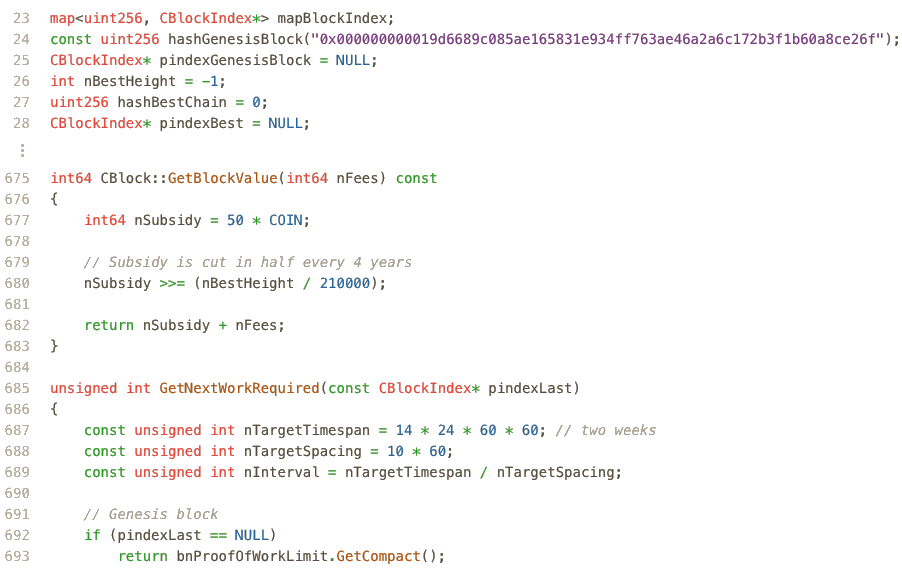
\includegraphics[width=\textwidth]{assets/images/bitcoin-code-white.png}
  \caption{Code excerpts from Bitcoin version 0.1}
  \label{fig:bitcoin-code-white}
\end{figure}

To make sure that his innovation transcends fantasy and becomes reality, Satoshi
wrote code to implement his idea before he wrote the whitepaper. He also made
sure not to delay\footnote{\enquote{We shouldn't delay forever until every possible
feature is done.} -- Satoshi Nakamoto~\cite{satoshi-delay}} any release forever.
After all, \enquote{there's always going to be one more thing to do.}

\begin{quotation}\begin{samepage}
\enquote{I had to write all the code before I could convince myself that I
could solve every problem, then I wrote the paper.}
\begin{flushright} -- Satoshi Nakamoto\footnote{Satoshi Nakamoto, Re: Bitcoin P2P e-cash paper \cite{satoshi-mail-code-first}}
\end{flushright}\end{samepage}\end{quotation}

In today's world of endless promises and doubtful execution, an exercise
in dedicated building was desperately needed. Be deliberate, convince
yourself that you can actually solve the problems, and implement the
solutions. We should all aim to be a bit more cypherpunk.

\paragraph{Bitcoin taught me that cypherpunks write code.}

% ---
%
% #### Down the Rabbit Hole
%
% - [Bitcoin version 0.1.0 announcement][version 0.1.0] by Satoshi Nakamoto
% - [Bitcoin P2P e-cash paper announcement][mail-announcement] by Satoshi Nakamoto
%
% [mail-announcement]: http://www.metzdowd.com/pipermail/cryptography/2008-October/014810.html
% [Ludwig Von Mises]: https://mises.org/library/human-action-0/html/pp/613
% [version 0.1.0]: https://bitcointalk.org/index.php?topic=68121.0
% [not to delay]: https://bitcointalk.org/index.php?topic=199.msg1670#msg1670
% [6]: http://www.metzdowd.com/pipermail/cryptography/2008-November/014832.html
%
% <!-- Wikipedia -->
% [alice]: https://en.wikipedia.org/wiki/Alice%27s_Adventures_in_Wonderland
% [carroll]: https://en.wikipedia.org/wiki/Lewis_Carroll

\chapter{Metaphors for Bitcoin's Future}
\label{les:21}

\begin{chapquote}{Lewis Carroll, \textit{Alice in Wonderland}}
\enquote{I know something interesting is sure to happen\ldots}
\end{chapquote}

In the last couple of decades, it became apparent that technological
innovation does not follow a linear trend. Whether you believe in the
technological singularity or not, it is undeniable that progress is
exponential in many fields. Not only that, but the rate at which
technologies are being adopted is accelerating, and before you know it
the bush in the local schoolyard is gone and your kids are using
Snapchat instead. Exponential curves have the tendency to slap you in
the face way before you see them coming.

Bitcoin is an exponential technology built upon exponential technologies.
\textit{Our World in Data}\footnote{\url{https://ourworldindata.org/}}
beautifully shows the rising speed of technological adoption, starting in 1903
with the introduction of landlines (see Figure~\ref{fig:tech-adoption}).
Landlines, electricity, computers, the internet, smartphones; all follow
exponential trends in price-performance and adoption. Bitcoin does
too~\cite{tech-adoption}.

\begin{center}
  \includegraphics[width=\textwidth]{assets/images/tech-adoption.png}
  \captionof{figure}{Bitcoin is literally off the charts.}
  \label{fig:tech-adoption}
\end{center}

Bitcoin has not one but multiple network effects\footnote{Trace Mayer,
\textit{The Seven Network Effects of Bitcoin}~\cite{7-network-effects}}, all of
which resulting in exponential growth patterns in their respective area: price,
users, security, developers, market share, and adoption as global money.

Having survived its infancy, Bitcoin is continuing to grow every day in
more aspects than one. Granted, the technology has not reached maturity
yet. It might be in its adolescence. But if the technology is
exponential, the path from obscurity to ubiquity is short.

\begin{center}
  \includegraphics[width=\textwidth]{assets/images/mobile-phone.png}
  \captionof{figure}{Mobile phone, ca 1965 vs 2019.}
  \label{fig:mobile-phone}
\end{center}

In his 2003 TED talk, Jeff Bezos chose to use electricity as a metaphor for the
web's future.\footnote{\url{http://bit.ly/bezos-web}} All three phenomena ---
electricity, the internet, Bitcoin --- are \textit{enabling} technologies,
networks which enable other things. They are infrastructure to be built upon,
foundational in nature.

Electricity has been around for a while now. We take it for granted. The
internet is quite a bit younger, but most people already take it for
granted as well. Bitcoin is ten years old and has entered public
consciousness during the last hype cycle. Only the earliest of adopters
take it for granted. As more time passes, more and more people will
recognize Bitcoin as something which simply is.\footnote{This is known as the
\textit{Lindy Effect}. The Lindy effect is a theory that the future life expectancy
of some non-perishable things like a technology or an idea is proportional to
their current age, so that every additional period of survival implies a longer
remaining life expectancy.~\cite{wiki:lindy}}

In 1994, the internet was still confusing and unintuitive. Watching this old
recording of the \textit{Today
Show}\footnote{\url{https://youtu.be/UlJku_CSyNg}} makes it obvious that what
feels natural and intuitive now actually wasn't back then. Bitcoin is still
confusing and alien to most, but just like the internet is second nature for
digital natives, spending and stacking
sats\footnote{\url{https://twitter.com/hashtag/stackingsats}} will be second
nature to the bitcoin natives of the future.

\begin{quotation}\begin{samepage}
\enquote{The future is already here --- it's just not very evenly
distributed.}
\begin{flushright} -- William Gibson\footnote{William Gibson, \textit{The Science in Science Fiction} \cite{william-gibson}}
\end{flushright}\end{samepage}\end{quotation}

In 1995, about $15\%$ of American adults used the internet. Historical
data from the Pew Research Center~\cite{pew-research} shows how the internet has woven
itself into all our lives. According to a consumer survey by Kaspersky
Lab~\cite{web:kaspersky}, 13\% of respondents have used Bitcoin and its clones to pay for
goods in 2018. While payments aren't the only use-case of bitcoin, it is
some indication of where we are in Internet time: in the early- to
mid-90s.

In 1997, Jeff Bezos stated in a letter to shareholders~\cite{bezos-letter} that
\enquote{this is Day 1 for the Internet,} recognizing the great untapped
potential for the internet and, by extension, his company. Whatever day this is
for Bitcoin, the vast amounts of untapped potential are clear to all but the
most casual observer.

\begin{center}
  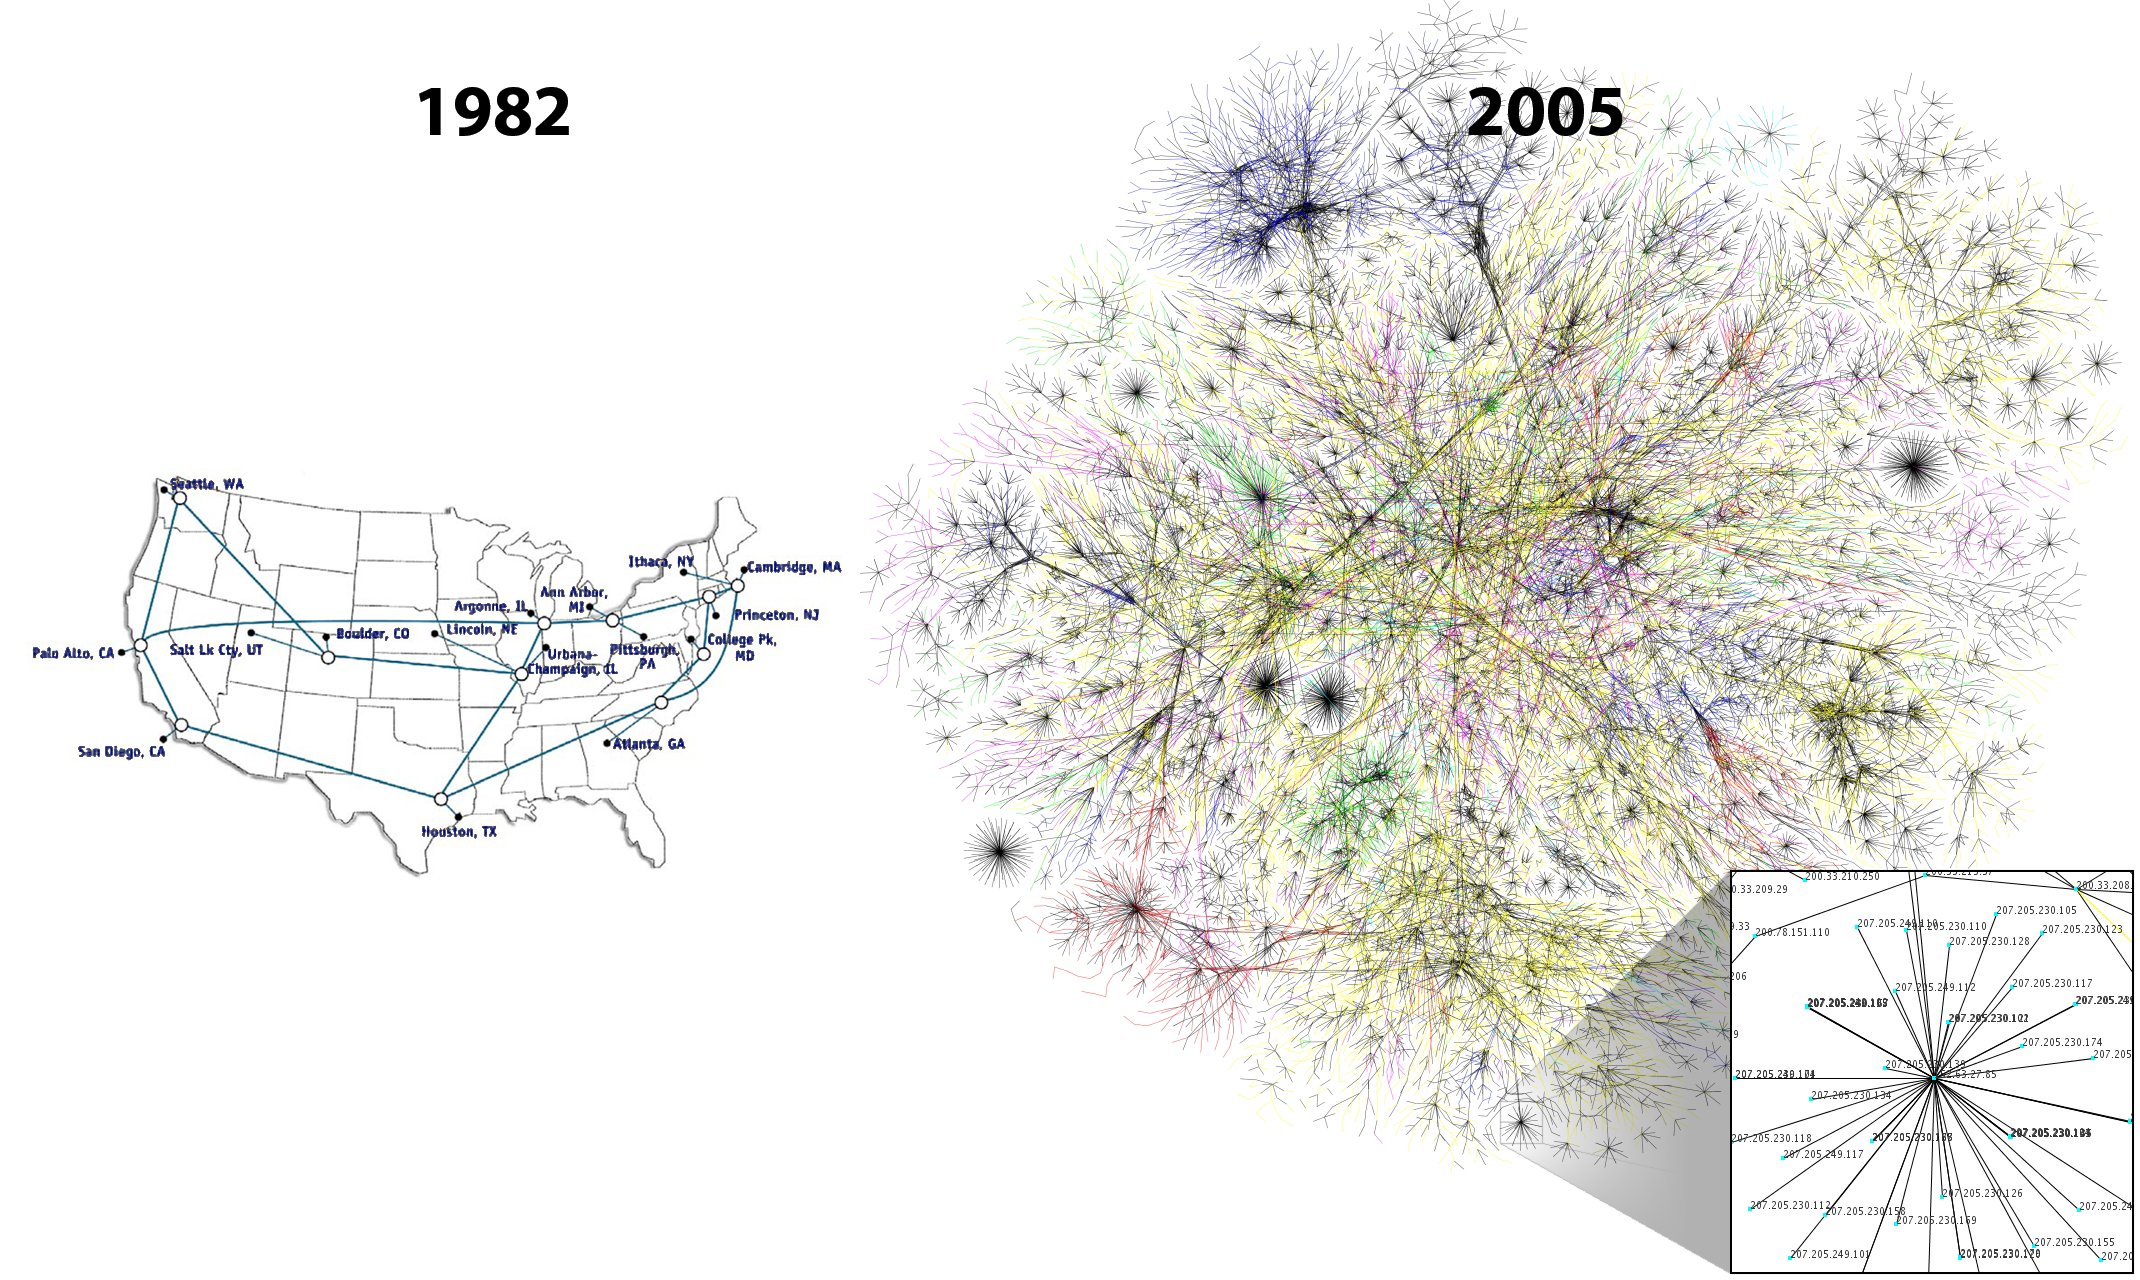
\includegraphics[width=\textwidth]{assets/images/internet-evolution-white-dates.png}
  \captionof{figure}{The internet, 1982 vs 2005. Source: cc-by Merit Network, Inc. and Barrett Lyon, Opte Project}
  \label{fig:internet-evolution-white-dates}
\end{center}

Bitcoin's first node went online in 2009 after Satoshi mined the \textit{genesis
block}\footnote{The genesis block is the first block of the Bitcoin block chain.
Modern versions of Bitcoin number it as block $0$, though very early versions
counted it as block $1$. The genesis block is usually hardcoded into the
software of the applications that utilize the Bitcoin block chain. It is a
special case in that it does not reference a previous block and produces an
unspendable subsidy. The \textit{coinbase} parameter contains, along with the
normal data, the following text: \textit{\enquote{The Times 03/Jan/2009 Chancellor on
brink of second bailout for banks}} \cite{btcwiki:genesis-block}} and released
the software into the wild. His node wasn't alone for long. Hal Finney was one
of the first people to pick up on the idea and join the network. Ten years
later, as of this writing, more than
$75.000$\footnote{\url{https://bit.ly/luke-nodecount}} nodes are running
bitcoin.

\begin{center}
  \centering
  \includegraphics[width=8cm]{assets/images/running-bitcoin.png}
  \captionof{figure}{Hal Finney authored the first tweet mentioning bitcoin in January 2009.}
  \label{fig:running-bitcoin}
\end{center}

The protocol's base layer isn't the only thing growing exponentially.
The lightning network, a second layer technology, is growing at an even
faster rate.

In January 2018, the lightning network had $40$ nodes and $60$
channels~\cite{web:lightning-nodes}. In April 2019, the network grew to more
than $4000$ nodes and around $40.000$ channels. Keep in mind that this is still
experimental technology where loss of funds can and does occur. Yet the trend is
clear: thousands of people are reckless and eager to use it.

\begin{center}
  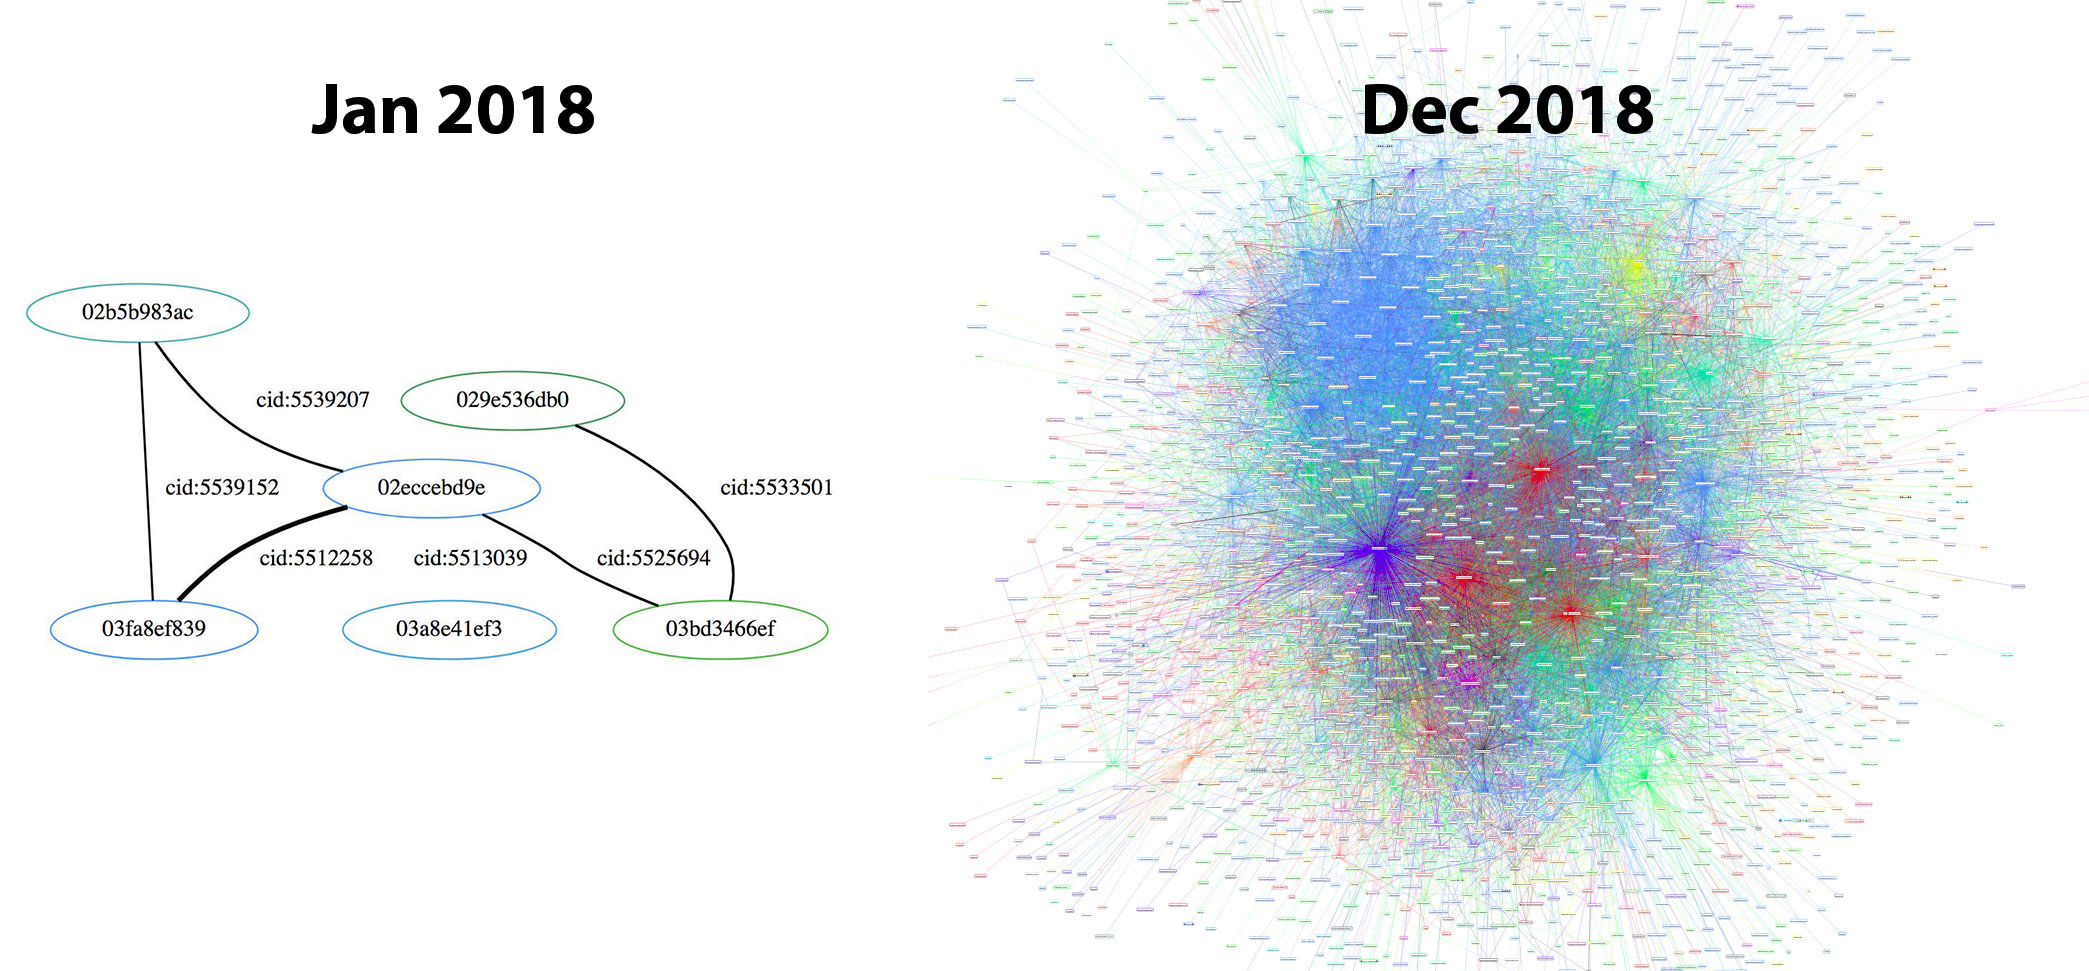
\includegraphics[width=\textwidth]{assets/images/lnd-growth-lopp-white.png}
  \captionof{figure}{Lightning Network, January 2018 vs December 2018. Source: Jameson Lopp}
  \label{fig:lnd-growth-lopp-white.png}
\end{center}

To me, having lived through the meteoric rise of the web, the parallels
between the internet and Bitcoin are obvious. Both are networks, both
are exponential technologies, and both enable new possibilities, new
industries, new ways of life. Just like electricity was the best
metaphor to understand where the internet is heading, the internet might
be the best metaphor to understand where bitcoin is heading. Or, in the
words of Andreas Antonopoulos, Bitcoin is \textit{The Internet of Money}.
These metaphors are a great reminder that while history doesn't repeat
itself, it often rhymes.

Exponential technologies are hard to grasp and often underestimated.
Even though I have a great interest in such technologies, I am
constantly surprised by the pace of progress and innovation. Watching
the Bitcoin ecosystem grow is like watching the rise of the internet in
fast-forward. It is exhilarating.

My quest of trying to make sense of Bitcoin has led me down the pathways
of history in more ways than one. Understanding ancient societal
structures, past monies, and how communication networks evolved were all
part of the journey. From the handaxe to the smartphone, technology has
undoubtedly changed our world many times over. Networked technologies
are especially transformational: writing, roads, electricity, the
internet. All of them changed the world. Bitcoin has changed mine and
will continue to change the minds and hearts of those who dare to use
it.

\paragraph{Bitcoin taught me that understanding the past is essential to
understanding its future. A future which is just beginning\ldots}

% ---
%
% #### Down the Rabbit Hole
%
% - [The Rising Speed of Technological Adoption][the rising speed of technological adoption] by Jeff Desjardins
% - [The 7 Network Effects of Bitcoin][multiple network effects] by Trace Mayer
% - [The Electricity Metaphor for the Web's Future][TED talk] by Jeff Bezos
% - [How the internet has woven itself into American life][data from the Pew Research Center] by Susannah Fox and Lee Rainie
% - [Genesis Block][genesis block] on the Bitcoin Wiki
% - [Lindy Effect][more time] on Wikipedia
%
% [Our World in Data]: https://ourworldindata.org/
% [the rising speed of technological adoption]: https://www.visualcapitalist.com/rising-speed-technological-adoption/
% [multiple network effects]: https://www.thrivenotes.com/the-7-network-effects-of-bitcoin/
% [TED talk]: https://www.ted.com/talks/jeff_bezos_on_the_next_web_innovation
% [recording of the Today Show]: https://www.youtube.com/watch?v=UlJku_CSyNg
% [William Gibson]: https://www.npr.org/2018/10/22/1067220/the-science-in-science-fiction
% [data from the Pew Research Center]: https://www.pewinternet.org/2014/02/27/part-1-how-the-internet-has-woven-itself-into-american-life/
% [consumer survey]: https://www.kaspersky.com/blog/money-report-2018/
% [letter to shareholders]: http://media.corporate-ir.net/media_files/irol/97/97664/reports/Shareholderletter97.pdf
% [running bitcoin]: https://twitter.com/halfin/status/1110302988?lang=en
% [40 nodes]: https://bitcoinist.com/bitcoin-lightning-network-mainnet-nodes/
% [reckless]: https://twitter.com/hashtag/reckless
% [Jameson Lopp]: https://twitter.com/lopp/status/1077200836072296449
% [\textit{The Internet of Money}]: https://theinternetofmoney.info/
% [stacking]: https://twitter.com/hashtag/stackingsats
%
% <!-- Bitcoin Wiki -->
% [genesis block]: https://en.bitcoin.it/wiki/Genesis_block
%
% <!-- Wikipedia -->
% [more time]: https://en.wikipedia.org/wiki/Lindy_effect
% [alice]: https://en.wikipedia.org/wiki/Alice%27s_Adventures_in_Wonderland
% [carroll]: https://en.wikipedia.org/wiki/Lewis_Carroll

\input{chapters/ch4-00-conclusion}

\cleardoublepage

\chapter*{Acknowledgments}
\pdfbookmark{Acknowledgments}{acknowledgments}

Thanks to the countless authors and content producers who influenced my thinking
on Bitcoin and the topics it touches. There are too many to list them all, but
I’ll do my best to name a few.

\begin{itemize}
  \item Thanks to Arjun Balaji for the tweet which motivated me to write this.
  \item Thanks to Marty Bent for providing endless food for thought and entertainment. If you are not subscribed to Marty’s Bent and Tales From The Crypt, you are missing out. Cheers Matt and Marty for guiding us through the rabbit hole.
  \item Thanks to Michael Goldstein and Pierre Rochard for curating and providing the greatest Bitcoin literature via the Nakamoto Institute. And thank you for creating the Noded Podcast which influenced my philosophical views on Bitcoin substantially.
  \item Thanks to Saifedean Ammous for his convictions, savage tweets, and writing The Bitcoin Standard
  \item Thanks to Francis Pouliot for sharing his excitement about finding out about the timechain.
  \item Thanks to Andreas M. Antonopoulos for all the educational material he has put out over the years.
  \item Thanks to Peter McCormack for his honest tweets and the What Bitcoin Did podcast, which keeps providing great insights from many areas of the space.
  \item Thanks to Jannik, Brandon, Matt, Camilo, Daniel, Michael, and Raphael for providing feedback to early drafts of some lessons. Special thanks to Jannik who proofread multiple drafts multiple times.
  \item Thanks to Dhruv Bansal and Matt Odell for taking the time to discuss some of these ideas with me.
  \item Thanks to Guy Swann for producing an audio version of 21lessons.com.
  \item Thanks to Friar Hass for his spiritual support and guidance, and for taking the time to write a foreword for this book.
  \item Thanks to my wife for putting up with me and my obsessive nature.
  \item Thanks to my family for supporting me during both the good times and the bad.
  \item Last but not least, thanks to all the bitcoin maximalists, shitcoin minimalists, shills, bots, and shitposters which reside in the beautiful garden that is Bitcoin twitter.
\end{itemize}

And finally, thank you for reading this. I hope you enjoyed it as much as I did enjoy writing it.


\listoffigures

\input{backmatter/bibliography}
\printbibliography
\theendnotes

\end{document}
